\casesection{Morphology in combination with weir}



\paragraph*{Purpose}
In this test the combination of morphology and weirs will be tested. 

\paragraph*{Linked claims}
Claims that are related to the current test case are:
\begin{itemize}
\item Morphology without bed-updating gives the same result as without morphology
\item Morphology runs in combination with weirs
\end{itemize}

\paragraph*{Approach}
The present test is designed is based on memoVersion{e02-f09-c020} for the simulation of the transitions between sub-critical and supercritical flow over a sub grid weir.


\paragraph*{Model description}

Two simple models have been tested, namely with structured and unstructured grids as shown in Figure \ref{fig:gridoverview}. These two models are investigated considering the following alternatives

\begin {itemize}
\item morphology with weir. Contraction coefficient of the weir equals 1.0. At the upstream boundary  bed level is slowly lowered in time.
\item morphology with weir.Contraction coefficient of the weir equals 1.0. At the upstream boundary  bed level is slowly lowered in time. But with the option \emph{BedUpd = false} and option \emph{BedLevType = 1}
\item morphology with weir.Contraction coefficient of the weir equals 1.0. At the upstream boundary  bed level is slowly lowered in time. But without morphology and option \emph{BedLevType = 1};
\end{itemize}

The initial bed level is a flat bed with the elevation of 11 m in both models. This tescases are run with constant Chezy friction of 65 m$^{1/2}$/s. 

A variable discharge at upstream boundary, varying from $0$ to about $69 m3/s$, and a constant downstream water level of $12.5$ m have been imposed (this has been taken from earlier testing case, so it is not clear why specifically this condition was used in earlier testing). 

It is to be noted that all test scenarios with morphology includes morphological boundary condition, i.e. bed level changes at the boundary (specified in $“*.bcm”$ file).  

In both models, two types input files for fixed weir have been used to check if there is any effect of different input. First type of weir input includes three columns with x, y and crest level, while second type includes 5 columns with additional two columns with parameters, referred to as sill depth at left and right side of the crest (this file is generated using DeltaShell). Besides, it seems that there is a parameter in $“*.mdu”$ file $“Sillheightmin”$ (as mentioned in the manual, the weir is treated only if the sill depth at both sides, i.e. 4th and 5th parameter in weir input file, is larger than this value).    

Remark: No changes have been made on flow and morphological conditions in these testing in the premise that these conditions appear to have been considered in earlier test cases. Although some conditions could be altered for current test simulations, for example related to varying discharge, morphological boundary condition, grid resolution etc.). 

\begin{figure}[h!]
\begin{center}
\begin{subfigure}[b]{0.7\textwidth}
\centering
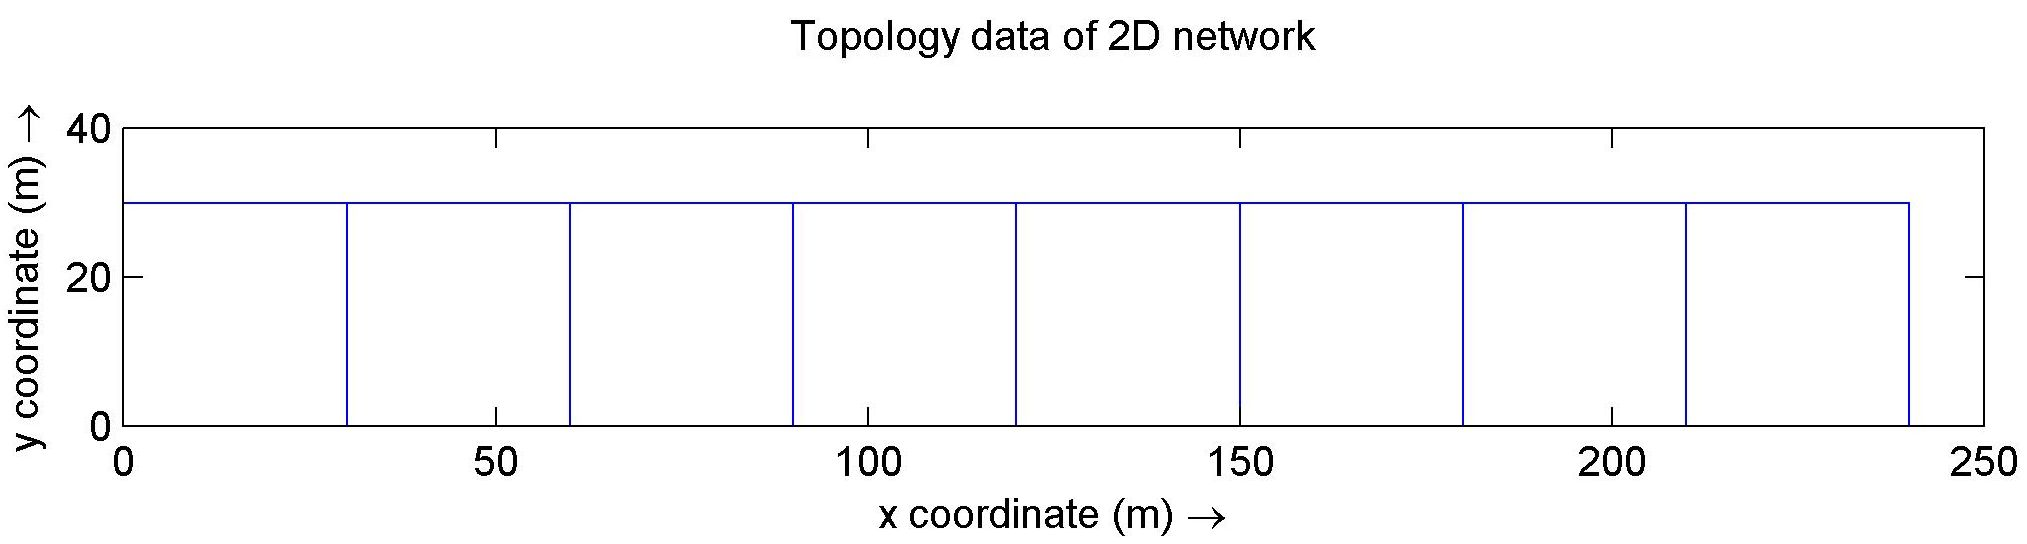
\includegraphics[width=0.8\columnwidth]{figures/Grid-rect.jpg} 
\end{subfigure}
\begin{subfigure}[b]{0.7\textwidth}
\centering
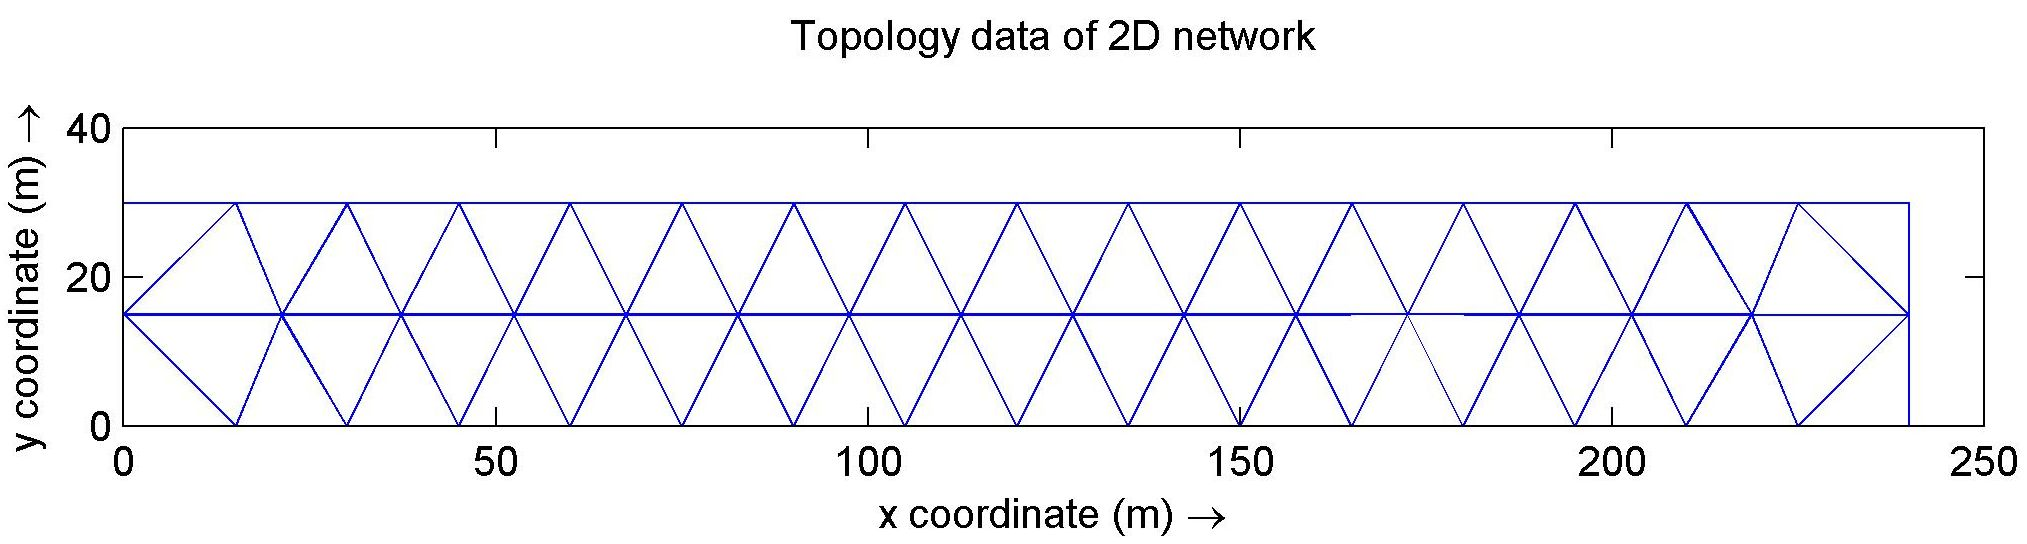
\includegraphics[width=0.8\columnwidth]{figures/Grid-triang.jpg} 
\end{subfigure}
\end{center}
\caption{Test models with structured (upper plot) and unstructured grid (lower plot) grids}
 \label{fig:gridoverview}
\end{figure}
\subparagraph*{Test Scenarios}
Following scenarios have been considered for model testing (all scenarios include weir): 
\begin {table} [H]
\caption {Scenarios setup} \label{tab:title1}
\begin{center}
	\begin{tabular} { |p{5cm} | p{5cm} |p{5cm} | }
		\hline
		{\bf Scenario No and detail} & {\bf General condition} & {\bf Weir condition} \\ \hline
		1=c16, sillheightmin = 0.5, sill depths = 10 & Model-Structured grid
		Bed level Type = 1 Hydrodynamics & Weir file generated from DeltaShell
		Sillheightmin  = 0.5 m (in $‘mdu’$ file) Right and left sill depths = 10 m  \\ \hline
		2=c15, sillheightmin = 0.5, sill depths = 10 & Model-Structured grid
		Bed level Type = 1 	Morphology with no bed level update (BedUpd = false in $‘*.mor’$ file) 
		 & Weir file generated from DeltaShell  Sillheightmin  = 0.5 m (in $‘mdu’$ file)
		 Right and left sill depths = 10 m 		  \\ 		\hline
		  
		3=c14, sillheightmin = 0.5, sill depths = 10 & Model-Structured grid
		Bed level Type = 1
		Morphology 		
		 &Weir file generated from DeltaShell
		 Sillheightmin  = 0.5 m (in $‘mdu’$ file)
		 Right and left sill depths = 10 m
		  \\ 		\hline
		4=c16, sillheightmin = 0.5, sill depths = 10 & Model-Unstructured grid
		Bed level Type = 1
		Hydrodynamics
		 & Weir file generated from DeltaShell
		 Sillheightmin  = 0.5 m (in $‘mdu’$ file)
		 Right and left sill depths = 10 m
		  \\ 		\hline
		5=c15, sillheightmin = 0.5, sill depths = 10 & Model-Unstructured grid
		Bed level Type = 1
		Morphology with no bed level update (BedUpd = false in $‘*.mor’$ file)
		 & Weir file generated from DeltaShell
		 Sillheightmin  = 0.5 m (in $‘mdu’$ file)
		 Right and left sill depths = 10 m
		  \\ 		\hline
		6=c14, sillheightmin = 0.5, sill depths = 10 & Model-Unstructured grid
		Bed level Type = 1
		Morphology
		 & Weir file generated from DeltaShell
		 Sillheightmin  = 0.5 m (in $‘mdu’$ file)
		 Right and left sill depths = 10 m
		 		  \\ 		\hline
		1w1=c16 & Model-Structured grid
		Bed level Type = 1
		Hydrodynamics
		 & Weir file with x,y and crest level only  \\ 		\hline
		2w1=c15 & Model-Structured grid
		Bed level Type = 1
		Morphology with no bed level update (BedUpd = false in $‘*.mor’$ file) 
		 & Weir file with x,y and crest level only \\ 		\hline
		3w1=c14 & Model-Structured grid
		Bed level Type = 1
		Morphology
		 &Weir file with x,y and crest level only  \\ 		\hline
		4w1=c16 unstructured & Model-Unstructured grid
		Bed level Type = 1
		Hydrodynamics
		 & Weir file with x,y and crest level only \\ 		\hline
		5w1=c15 unstructur & Model-Unstructured grid
		Bed level Type = 1
		Morphology with no bed level update (BedUpd = false in $‘*.mor’$ file)
		 & Weir file with x,y and crest level only \\ 		\hline
	
		 
			\end{tabular}
		\end{center}
	\end{table} 
		 
		 
		 
	\begin {table} [H]
	\caption { Continue scenarios setup} \label{tab:title2}
	\begin{center}
		\begin{tabular} { |p{5cm} | p{5cm} |p{5cm} | }
			\hline
			{\bf Scenario No and detail} & {\bf General condition} & {\bf Weir condition} \\ \hline	 
		 
		 6w1=c14 unstructured & Model-Unstructured grid
		 	Bed level Type = 1
		 	Morphology
		 	& Weir file with x,y and crest level only \\ 		\hline
		1w2=c16, sillheightmin = 0, sill depths = 0  & Model-Structured grid
		Bed level Type = 1
		Hydrodynamics
		 & Weir file generated from DeltaShell
		 Sillheightmin  = 0 m (in $‘mdu’$ file)
		 Right and left sill depths = 0 m
		  \\ 		\hline
		1w3=c16, sillheightmin = 0.5, sill depths = 0 & Model-Structured grid
		Bed level Type = 1
		Hydrodynamics
		 & Weir file generated from DeltaShell
		 Sillheightmin  = 0.5 m (in $‘mdu’$ file)
		 Right and left sill depths = 0 m
		 
		  \\ 		\hline
		2w2=c15, sillheightmin = 0, sill depths = 0 & Model-Structured grid
		Bed level Type = 1
		Morphology with no bed level update (BedUpd = false in $‘*.mor’$ file)
		 & Weir file generated from DeltaShell
		 Sillheightmin  = 0 m (in $‘mdu’$ file)
		 Right and left sill depths = 0 m
		  \\ 		\hline
		3w2=c14, sillheightmin = 0, sill depths = 0 & Model-Structured grid
		Bed level Type = 1
		Morphology
		 & Weir file generated from DeltaShell
		 Sillheightmin  = 0 m (in $‘mdu’$ file)
		 Right and left sill depths = 0 m
		  \\ 		\hline
		3w3=c14, sillheightmin = 0.5, sill depths = 0 & Model-Structured grid
		Bed level Type = 1
		Morphology
		 & Weir file generated from DeltaShell
		 Sillheightmin  = 0.5 m (in $‘mdu’$ file)
		 Right and left sill depths = 0 m
		  \\ 		\hline
		4w2=c16, sillheightmin = 0, silldepths = 0  & Model-Unstructured grid
		Bed level Type = 1
		Hydrodynamics
		 & Weir file generated from DeltaShell
		 Sillheightmin  = 0 m (in $‘mdu’$ file)
		 Right and left sill depths = 0 m
		  \\ 		\hline
		4w3=c16, sillheightmin = 0.5, sill depths = 0 & Model-Unstructured grid
		Bed level Type = 1
		Hydrodynamics
		 & Weir file generated from DeltaShell
		 Sillheightmin  = 0.5 m (in $‘mdu’$ file)
		 Right and left sill depths = 0 m
		  \\ 		\hline
		6w2=c14, sillheightmin = 0, sill depths = 0 & Model-Unstructured grid
		Bed level Type = 1
		Morphology
		 & Weir file generated from DeltaShell
		 Sillheightmin  = 0 m (in $‘mdu’$ file)
		 Right and left sill depths = 0 m
		  \\ 		\hline
		6w3=c14, sillheightmin = 0.5, sill depths = 0 & Model-Unstructured grid
		Bed level Type = 1
		Morphology
		 & Weir file generated from DeltaShell
		 Sillheightmin  = 0.5 m (in $‘mdu’$ file)
		 Right and left sill depths = 0 m
		  \\ 		\hline
				
		

	\end{tabular}
\end{center}
\end{table}
%\begin{tabu}  to 0.8\textwidth { | X[l] | X[c] | X[r] | }
%\hline
%Scenario No & General Conditions & Weir conditions \\
%\hline
%item 21  & item 22  & item 23  \\
%\hline
%\end{tabu}

Notes: Following are the coordinates of the slices, used for plotting longitudinal profiles: 
\begin{itemize}
\item $0.953, 14.356; 239.906, 15.214$ (middle).
\item $0.953, 23.365; 239.477, 23.365$ (left).
\item $2.240, 5.776; 239.477, 6.634$ (right).

\end{itemize}
\begin{figure}[h!]
\begin{center}
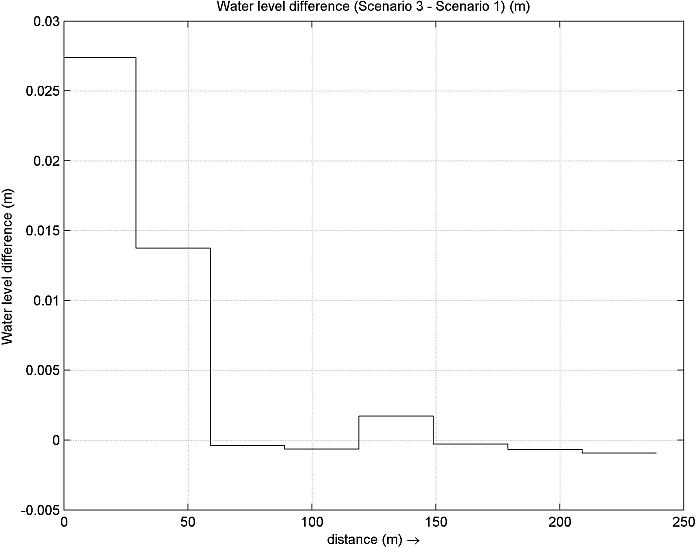
\includegraphics[width=0.8\columnwidth]{figures/WL-Sc3-Sc1.jpg} 
\end{center}\caption{Difference in water levels (longitudinal profile) between hydrodynamic and morphological simulations for the model with structured grid \label{fig:1.2}}
\end{figure}

\begin{figure}[h!]
\begin{center}
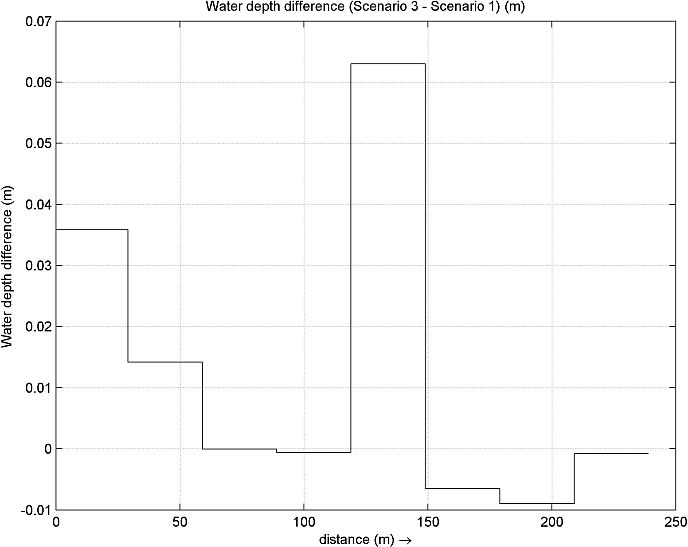
\includegraphics[width=0.8\columnwidth]{figures/depth-Sc3-Sc1.jpg} 
\end{center}\caption{Difference in water depth (longitudinal profile) between hydrodynamic and morphological simulations for the model with structured grid \label{fig:1.3}}
\end{figure}

\begin{figure}[h!]
	\begin{center}
		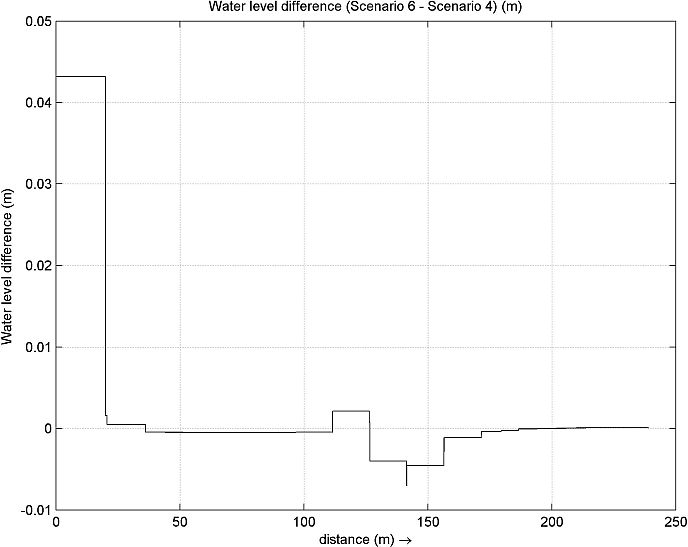
\includegraphics[width=0.8\columnwidth]{figures/WL-Sc6-Sc4.jpg} 
	\end{center}\caption{Difference in water depth (longitudinal profile) between hydrodynamic and morphological simulations for the model with structured grid \label{fig:1.4}}
\end{figure}

\begin{figure}[h!]
	\begin{center}
		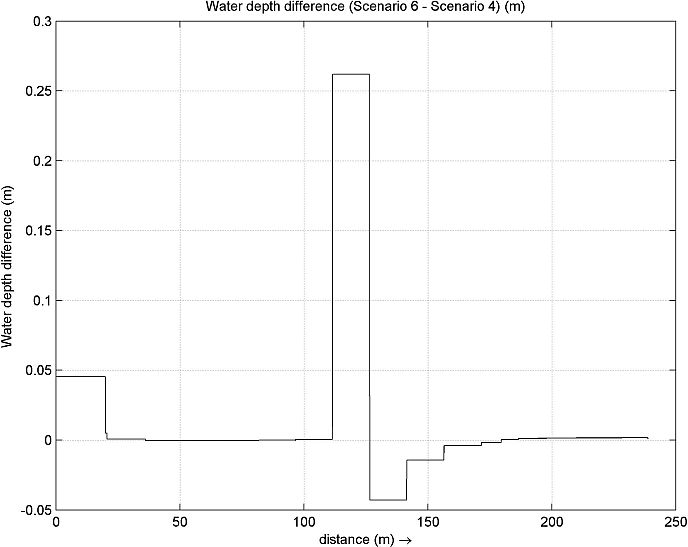
\includegraphics[width=0.8\columnwidth]{figures/depth-Sc6-Sc4.jpg} 
	\end{center}\caption{Difference in water depth (longitudinal profile) between hydrodynamic and morphological simulations for the model with unstructured grid \label{fig:1.5}}
\end{figure}

\begin{figure}[h!]
	\begin{center}
		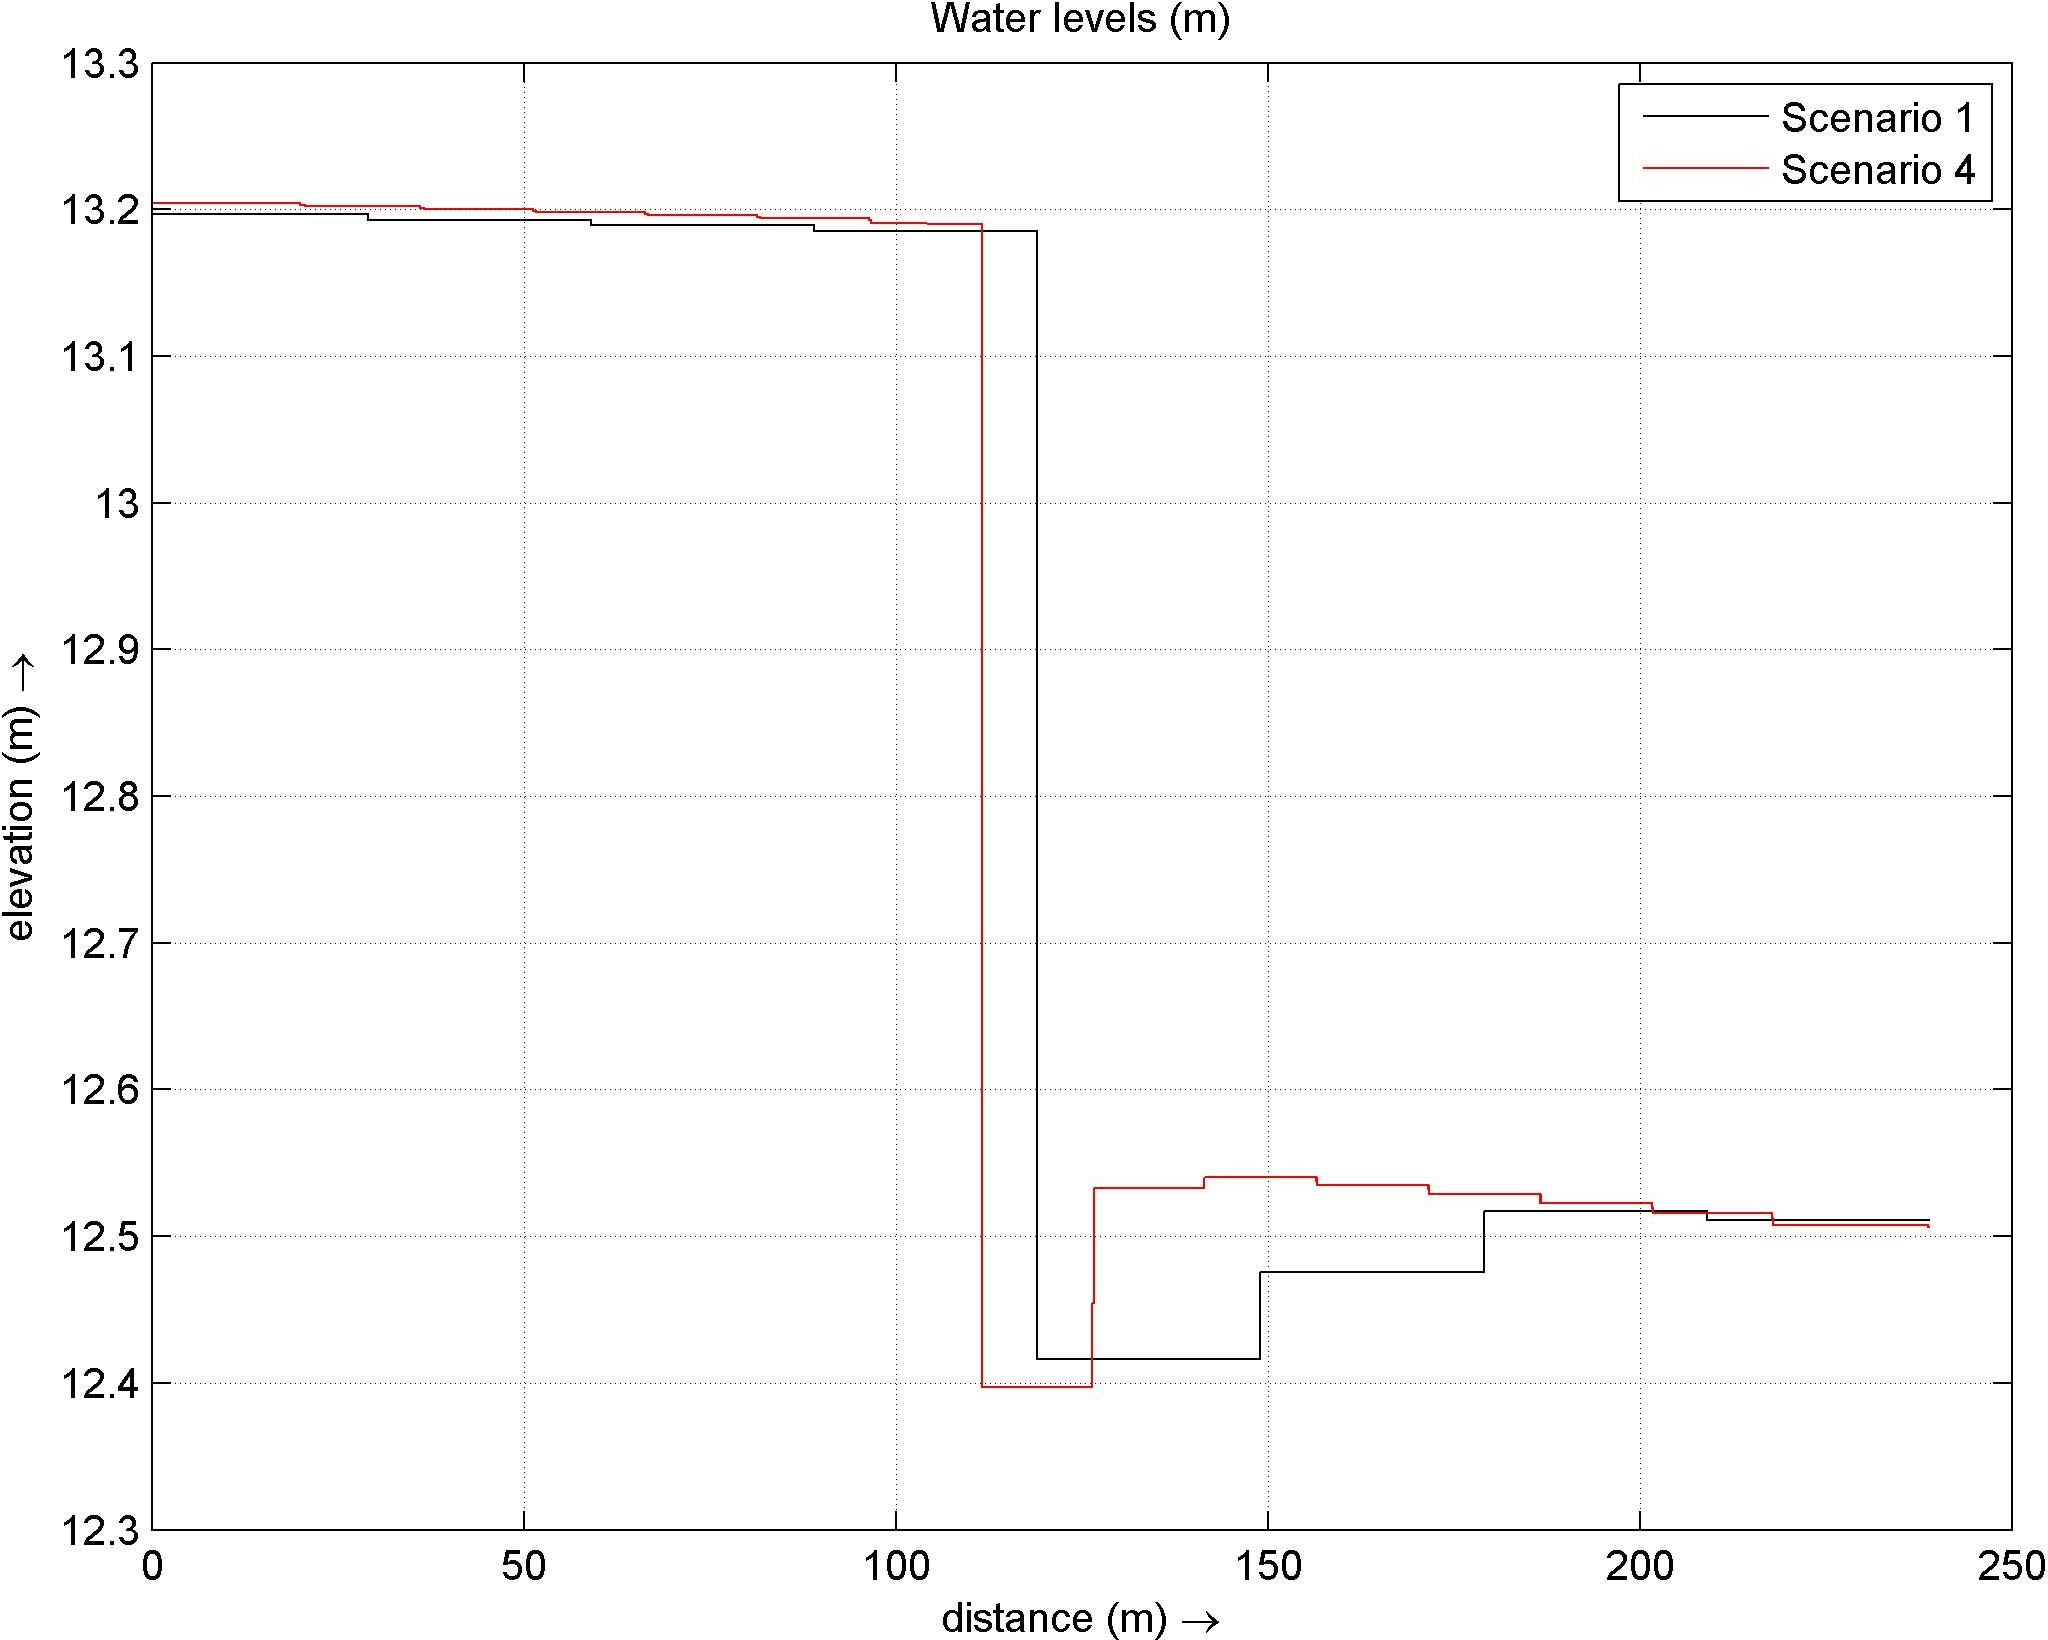
\includegraphics[width=0.8\columnwidth]{figures/WL-Sc1Sc4.jpg} 
	\end{center}\caption{Longitudinal water level profiles: Comparison between the results, predicted by the models with structured and unstructured grid (hydrodynamic simulations) \label{fig:1.6}}
\end{figure}

\begin{figure}[h!]
	\begin{center}
		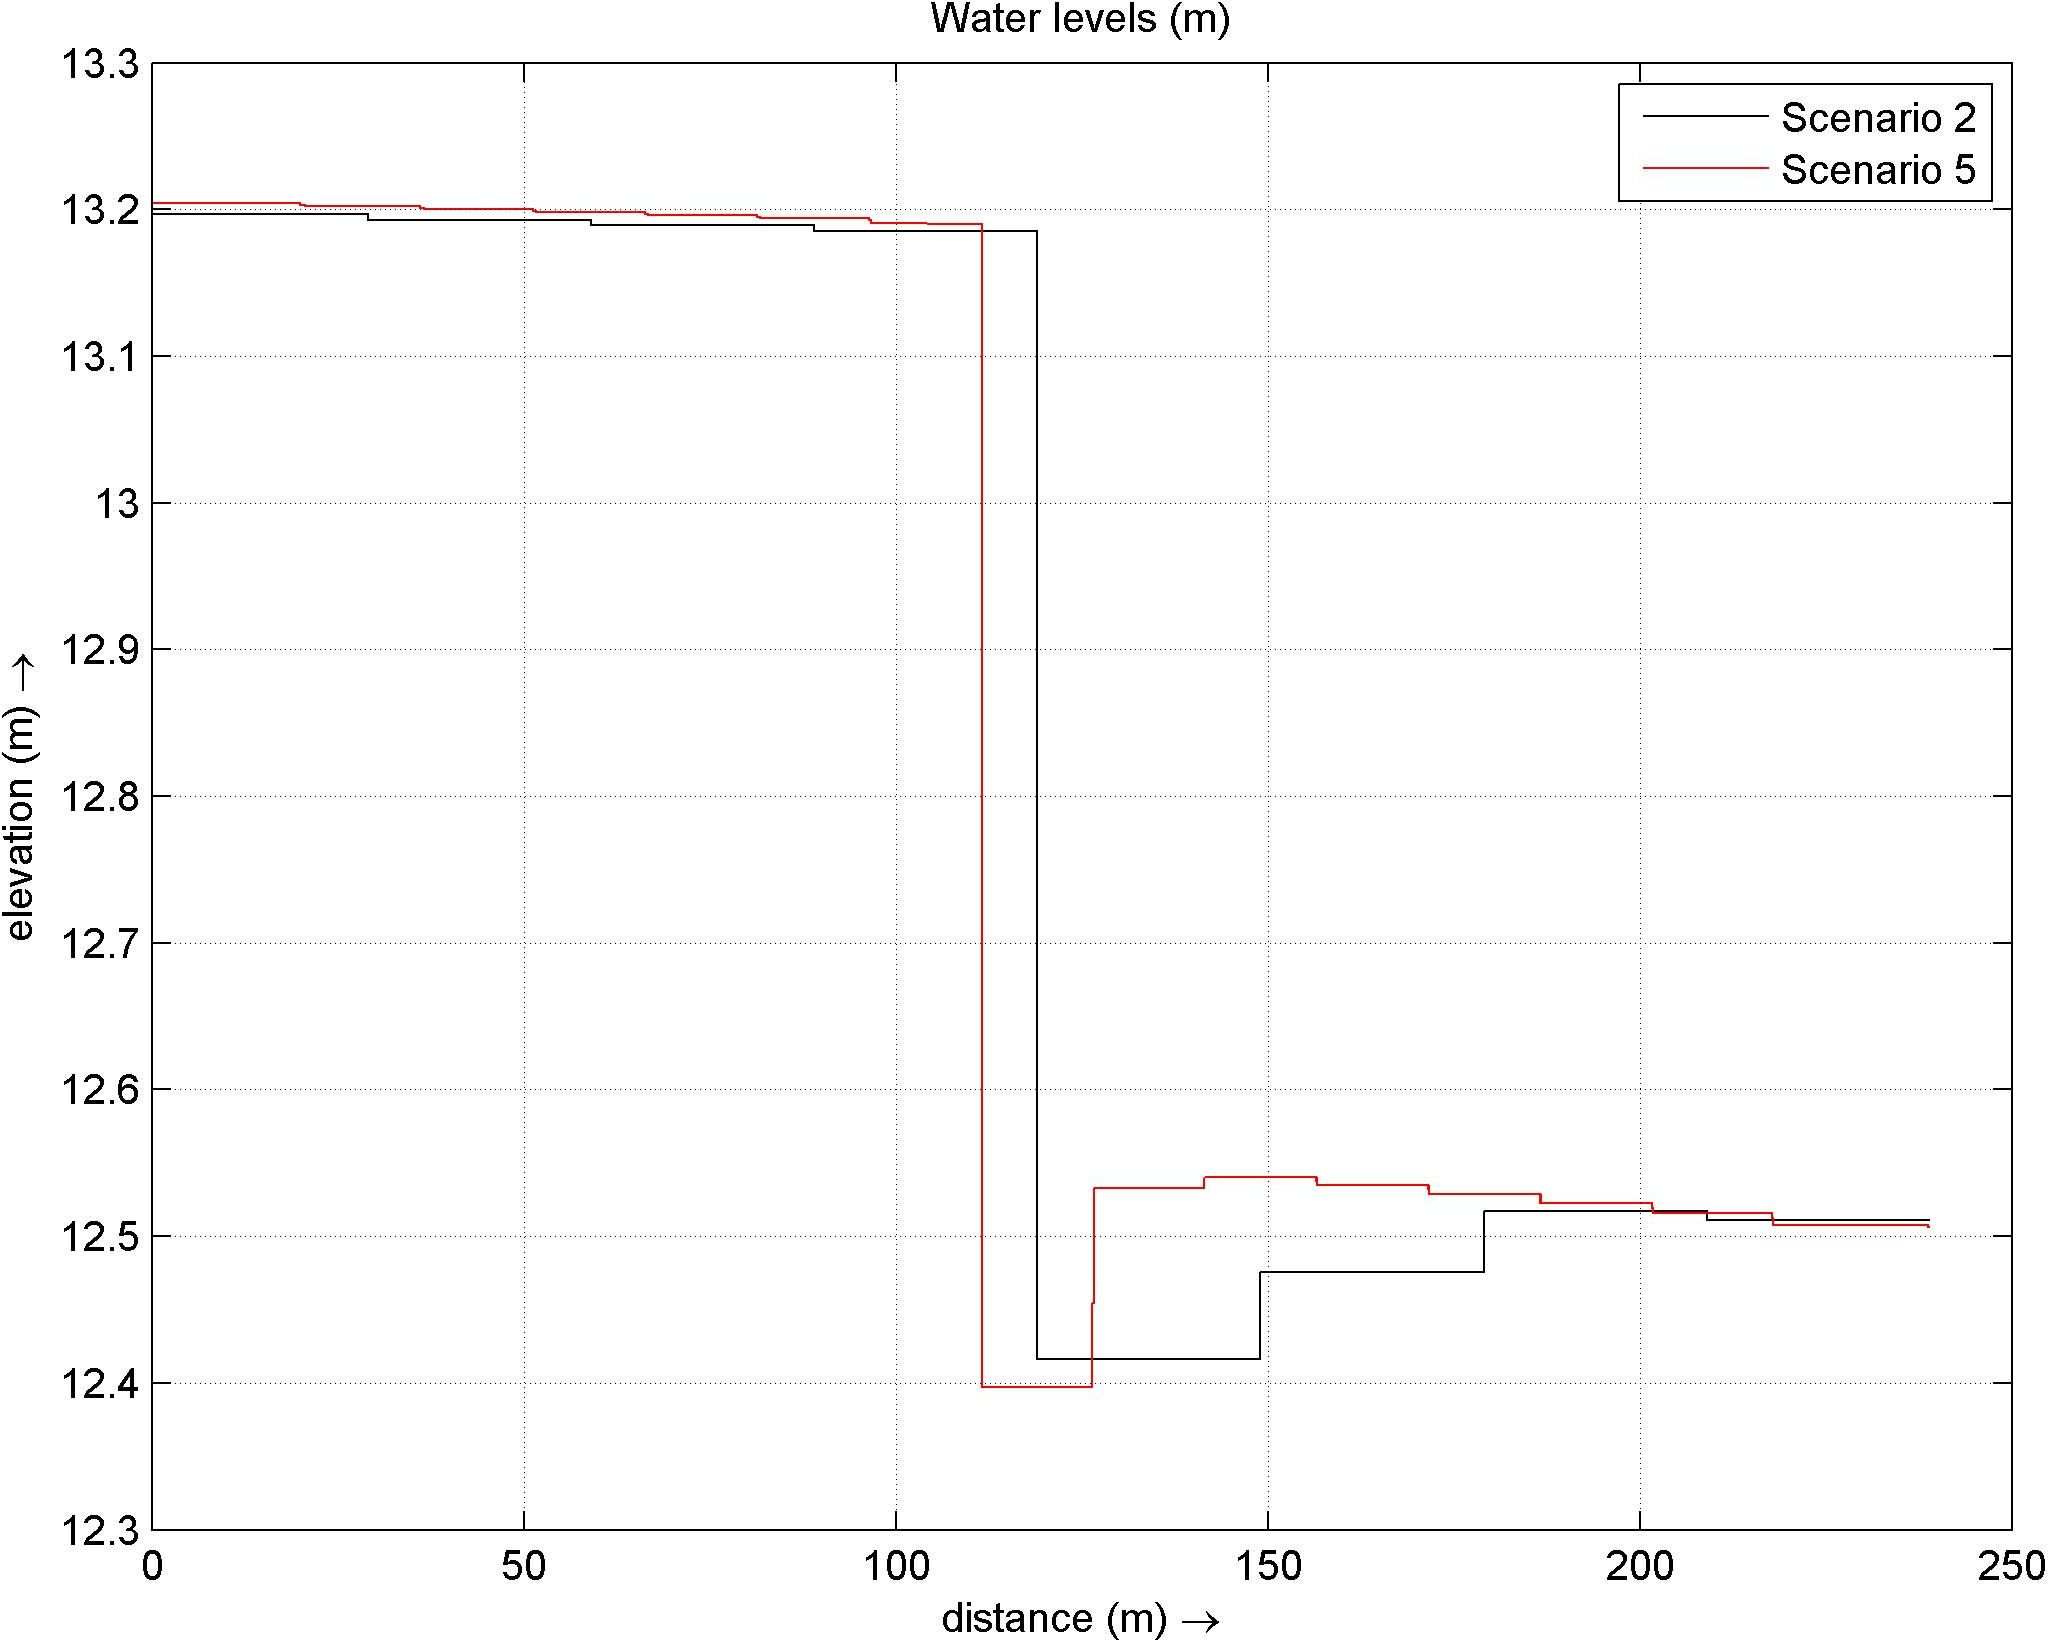
\includegraphics[width=0.8\columnwidth]{figures/WL-Sc2Sc5.jpg} 
	\end{center}\caption{Longitudinal water level profiles: Comparison between the results, predicted by the models with structured and unstructured grid (morphological simulations with no bed update condition) \label{fig:1.7}}
\end{figure}

\begin{figure}[h!]
	\begin{center}
		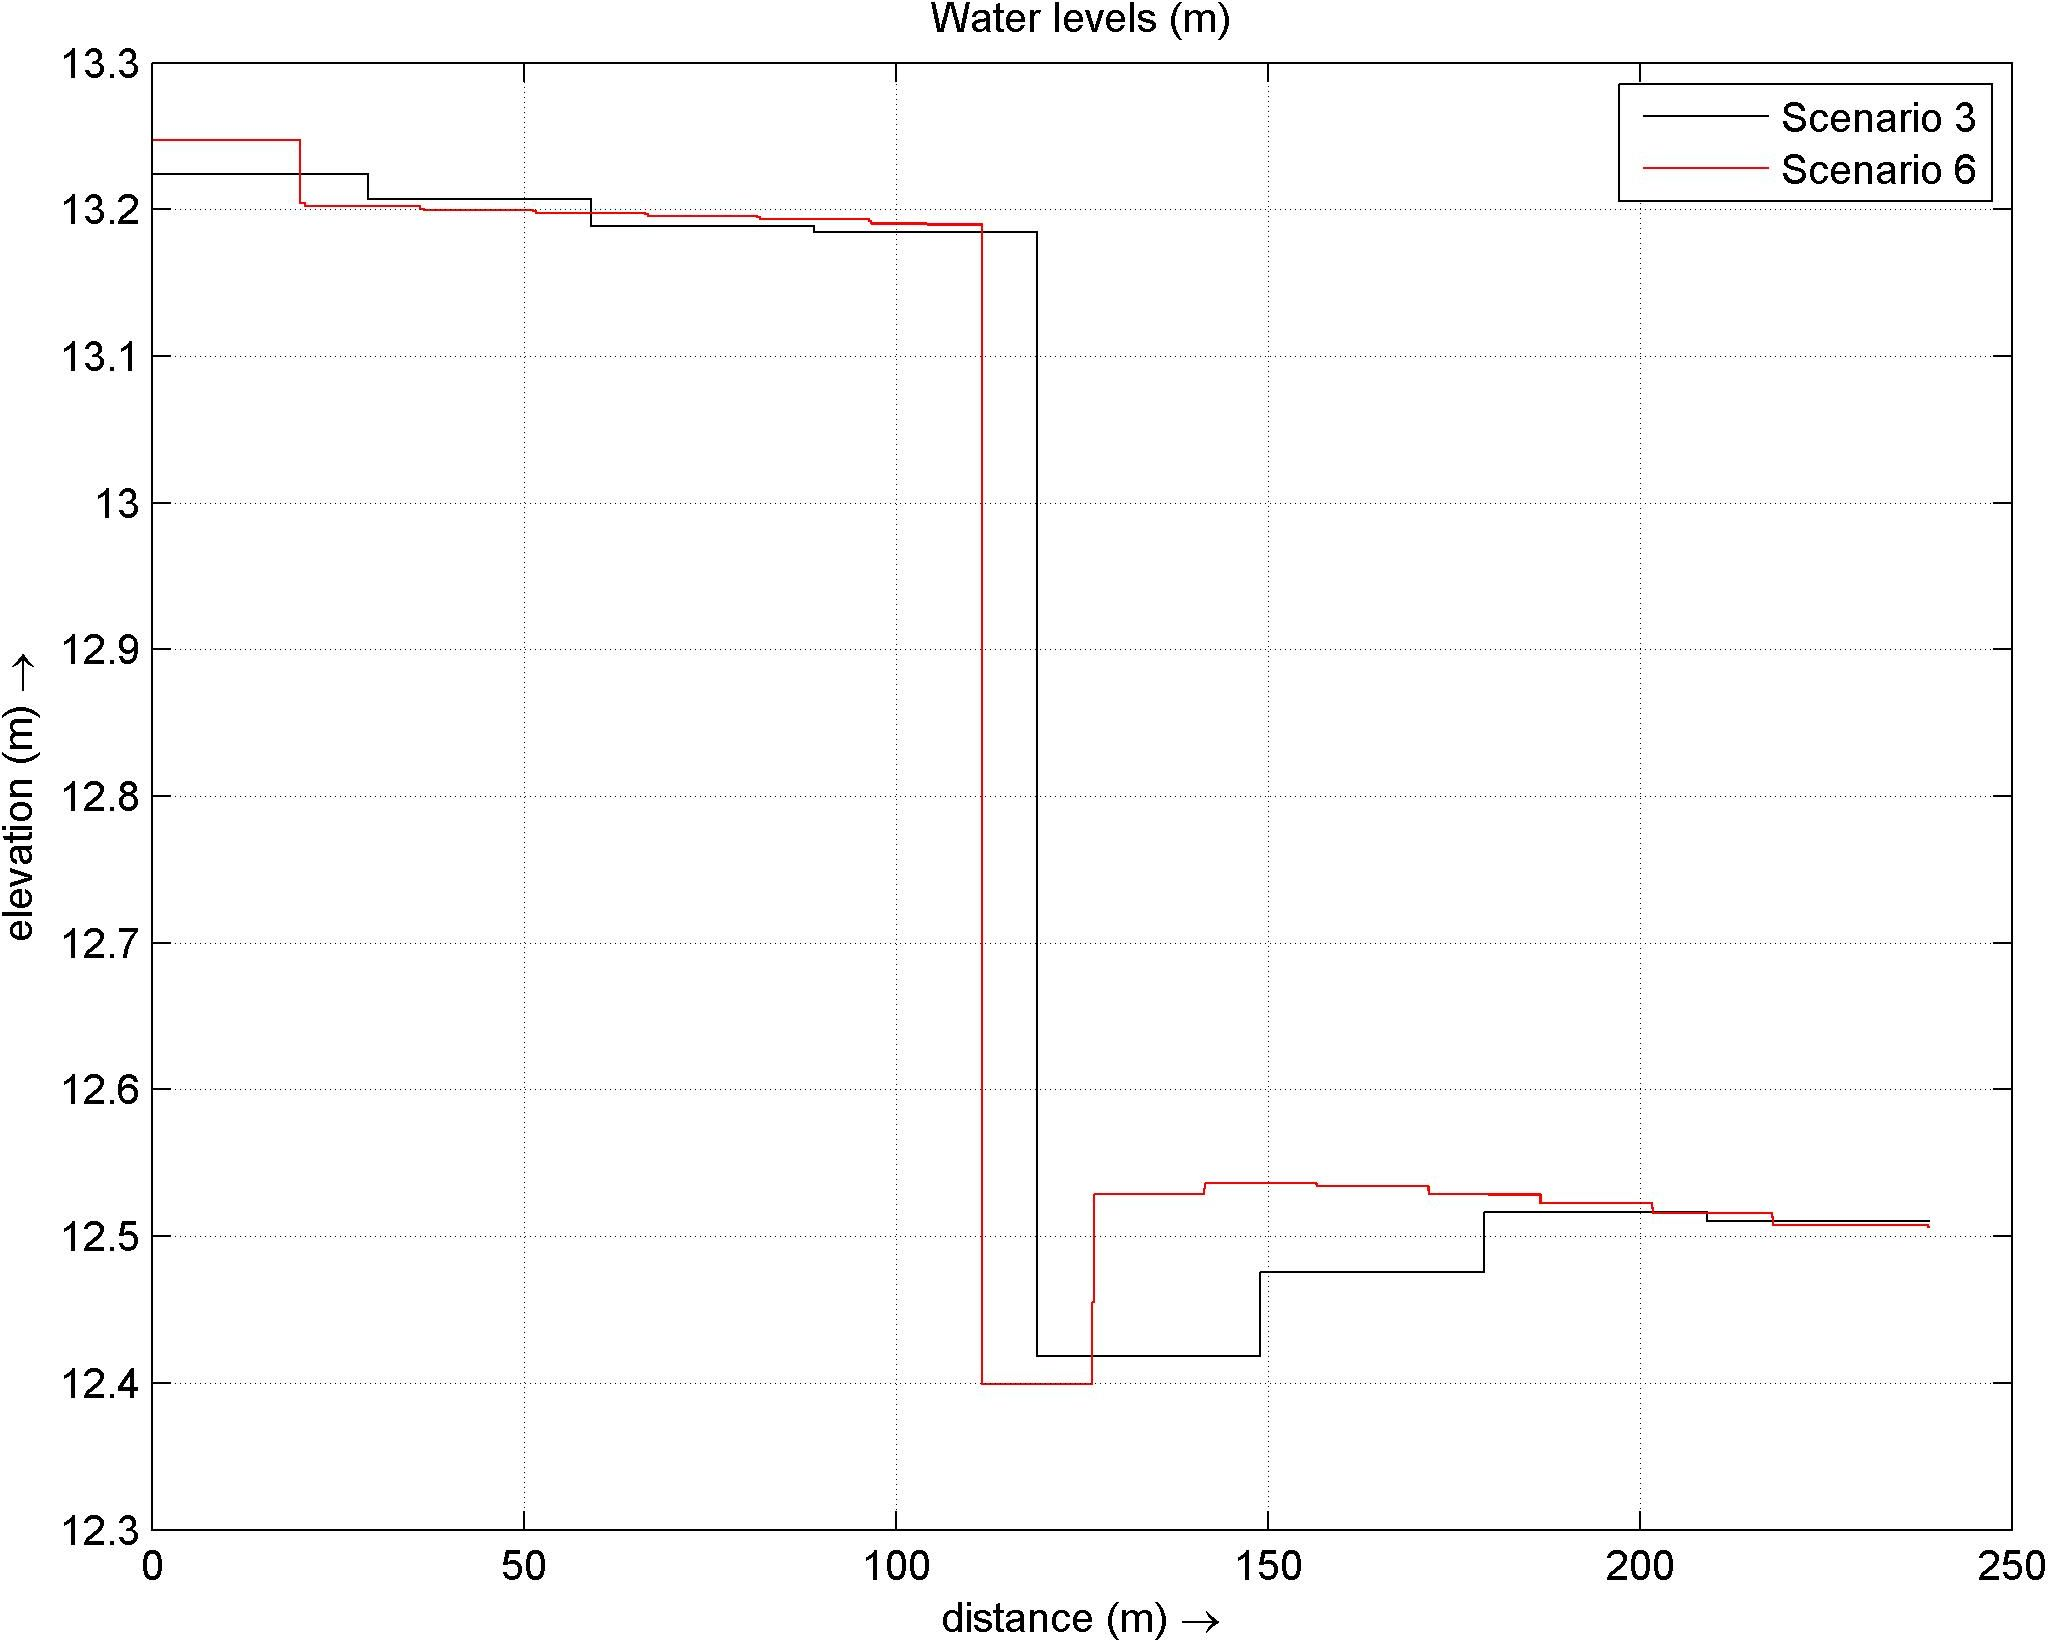
\includegraphics[width=0.8\columnwidth]{figures/WL-Sc3Sc6.jpg} 
	\end{center}\caption{Longitudinal water level profiles: Comparison between the results, predicted by the models with structured and unstructured grid (morphological simulations)	 \label{fig:1.8}}
\end{figure}

\begin{figure}[h!]
	\begin{center}
		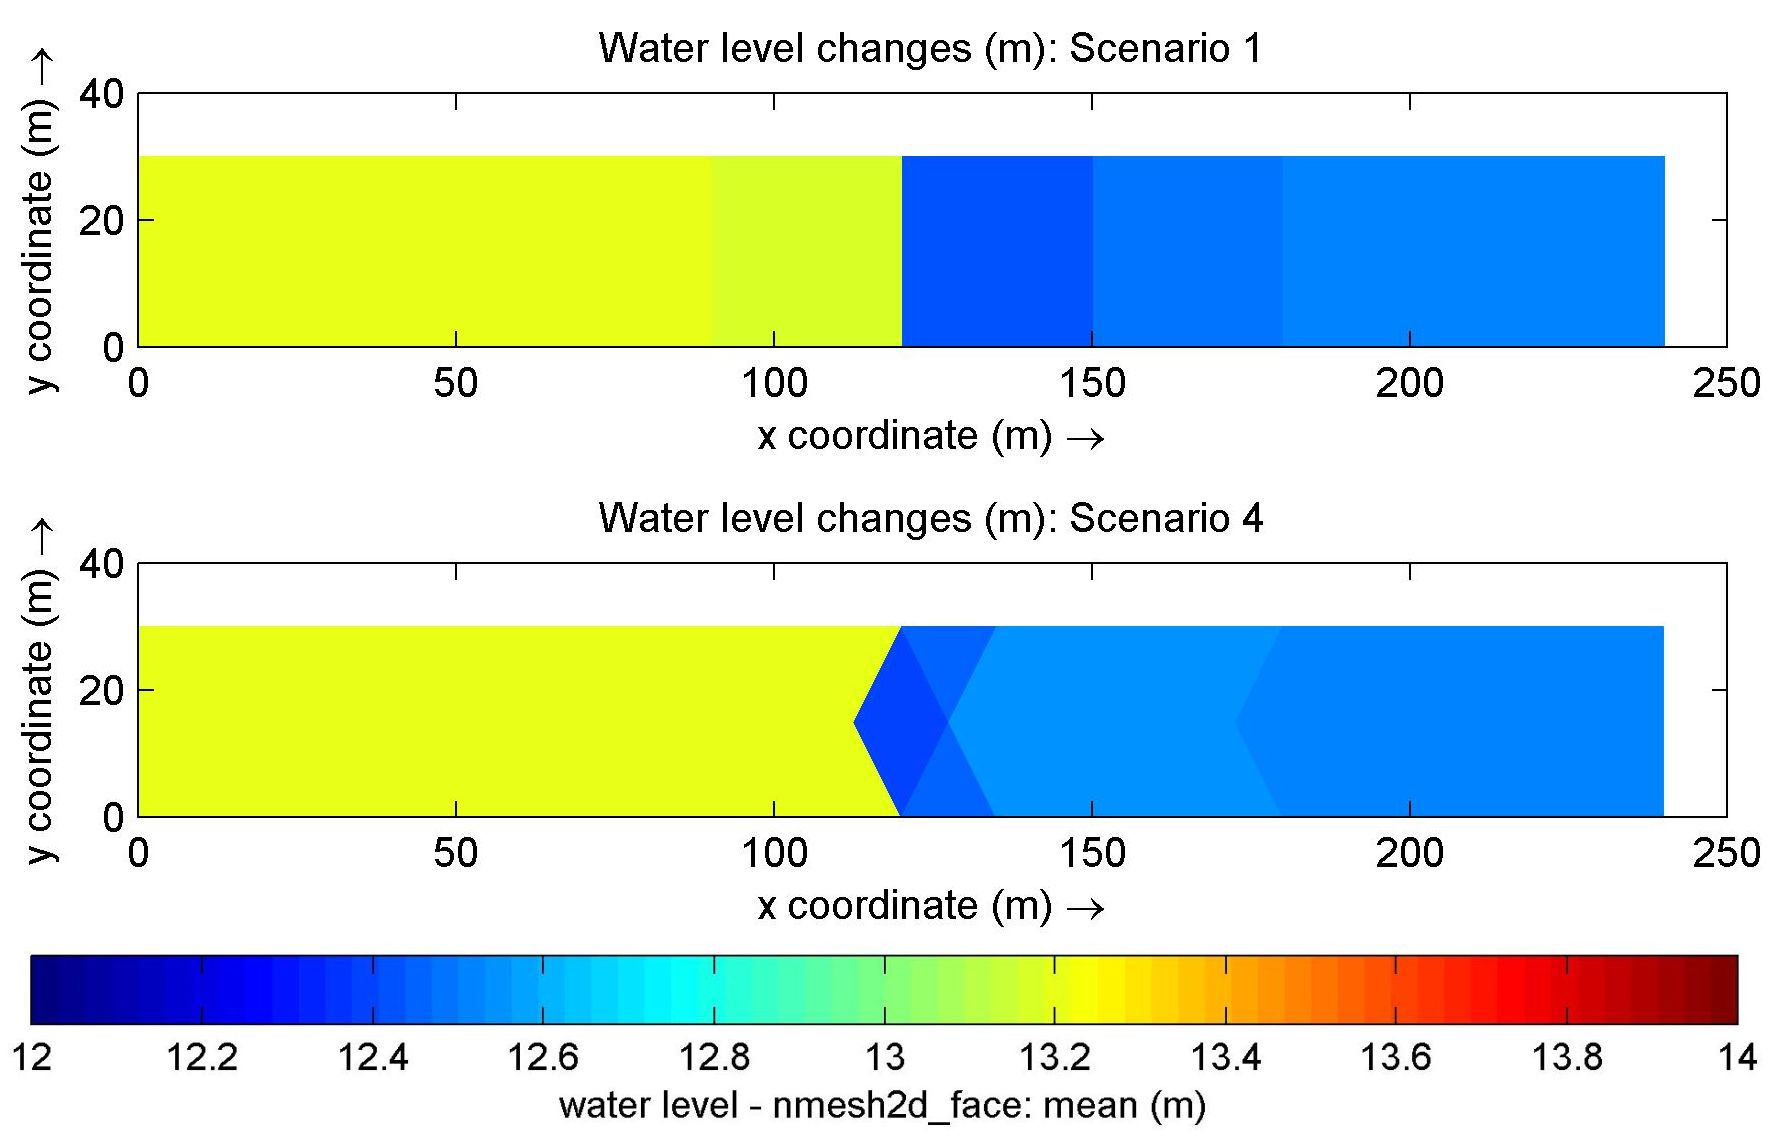
\includegraphics[width=0.8\columnwidth]{figures/WL-combined.jpg} 
	\end{center}\caption{Water level plots for structured (upper plot) and unstructured (lower plot) grid, showing also the projection of the weir \label{fig:1.9}}
\end{figure}

\begin{figure}[h!]
\begin{center}
	\begin{subfigure}[b]{0.7\textwidth}
		\centering
		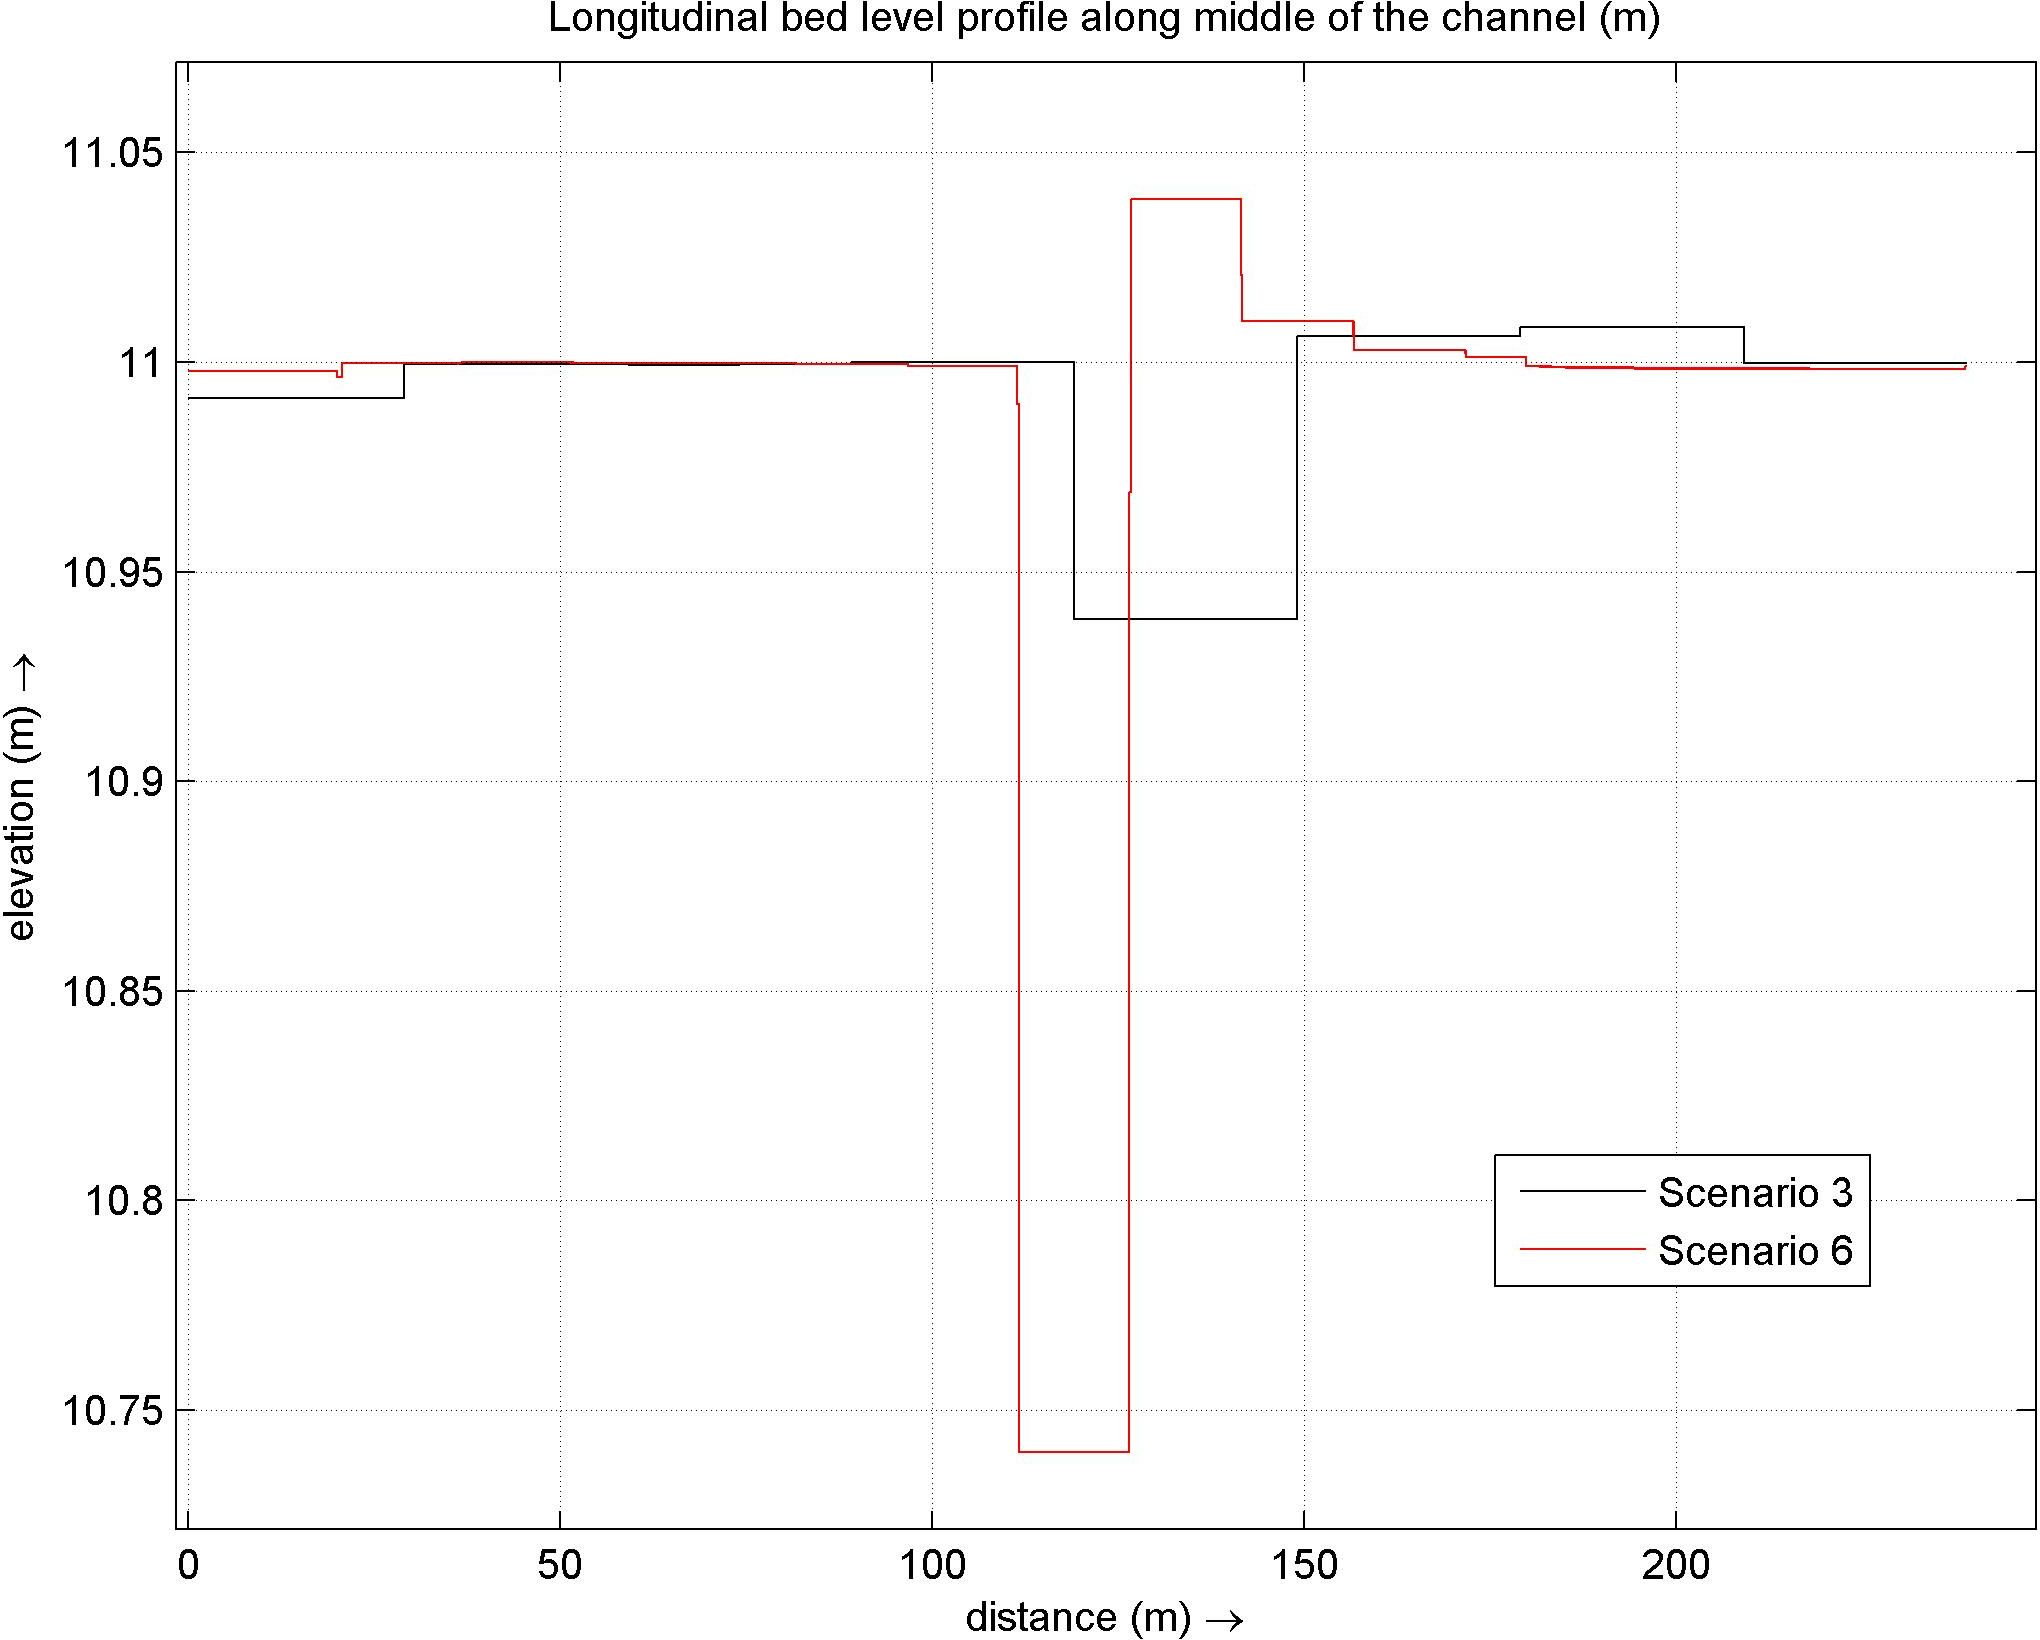
\includegraphics[width=0.8\columnwidth]{figures/BedlevelSc3-6-middle.jpg} 
	\end{subfigure}
	\begin{subfigure}[b]{0.7\textwidth}
		\centering
		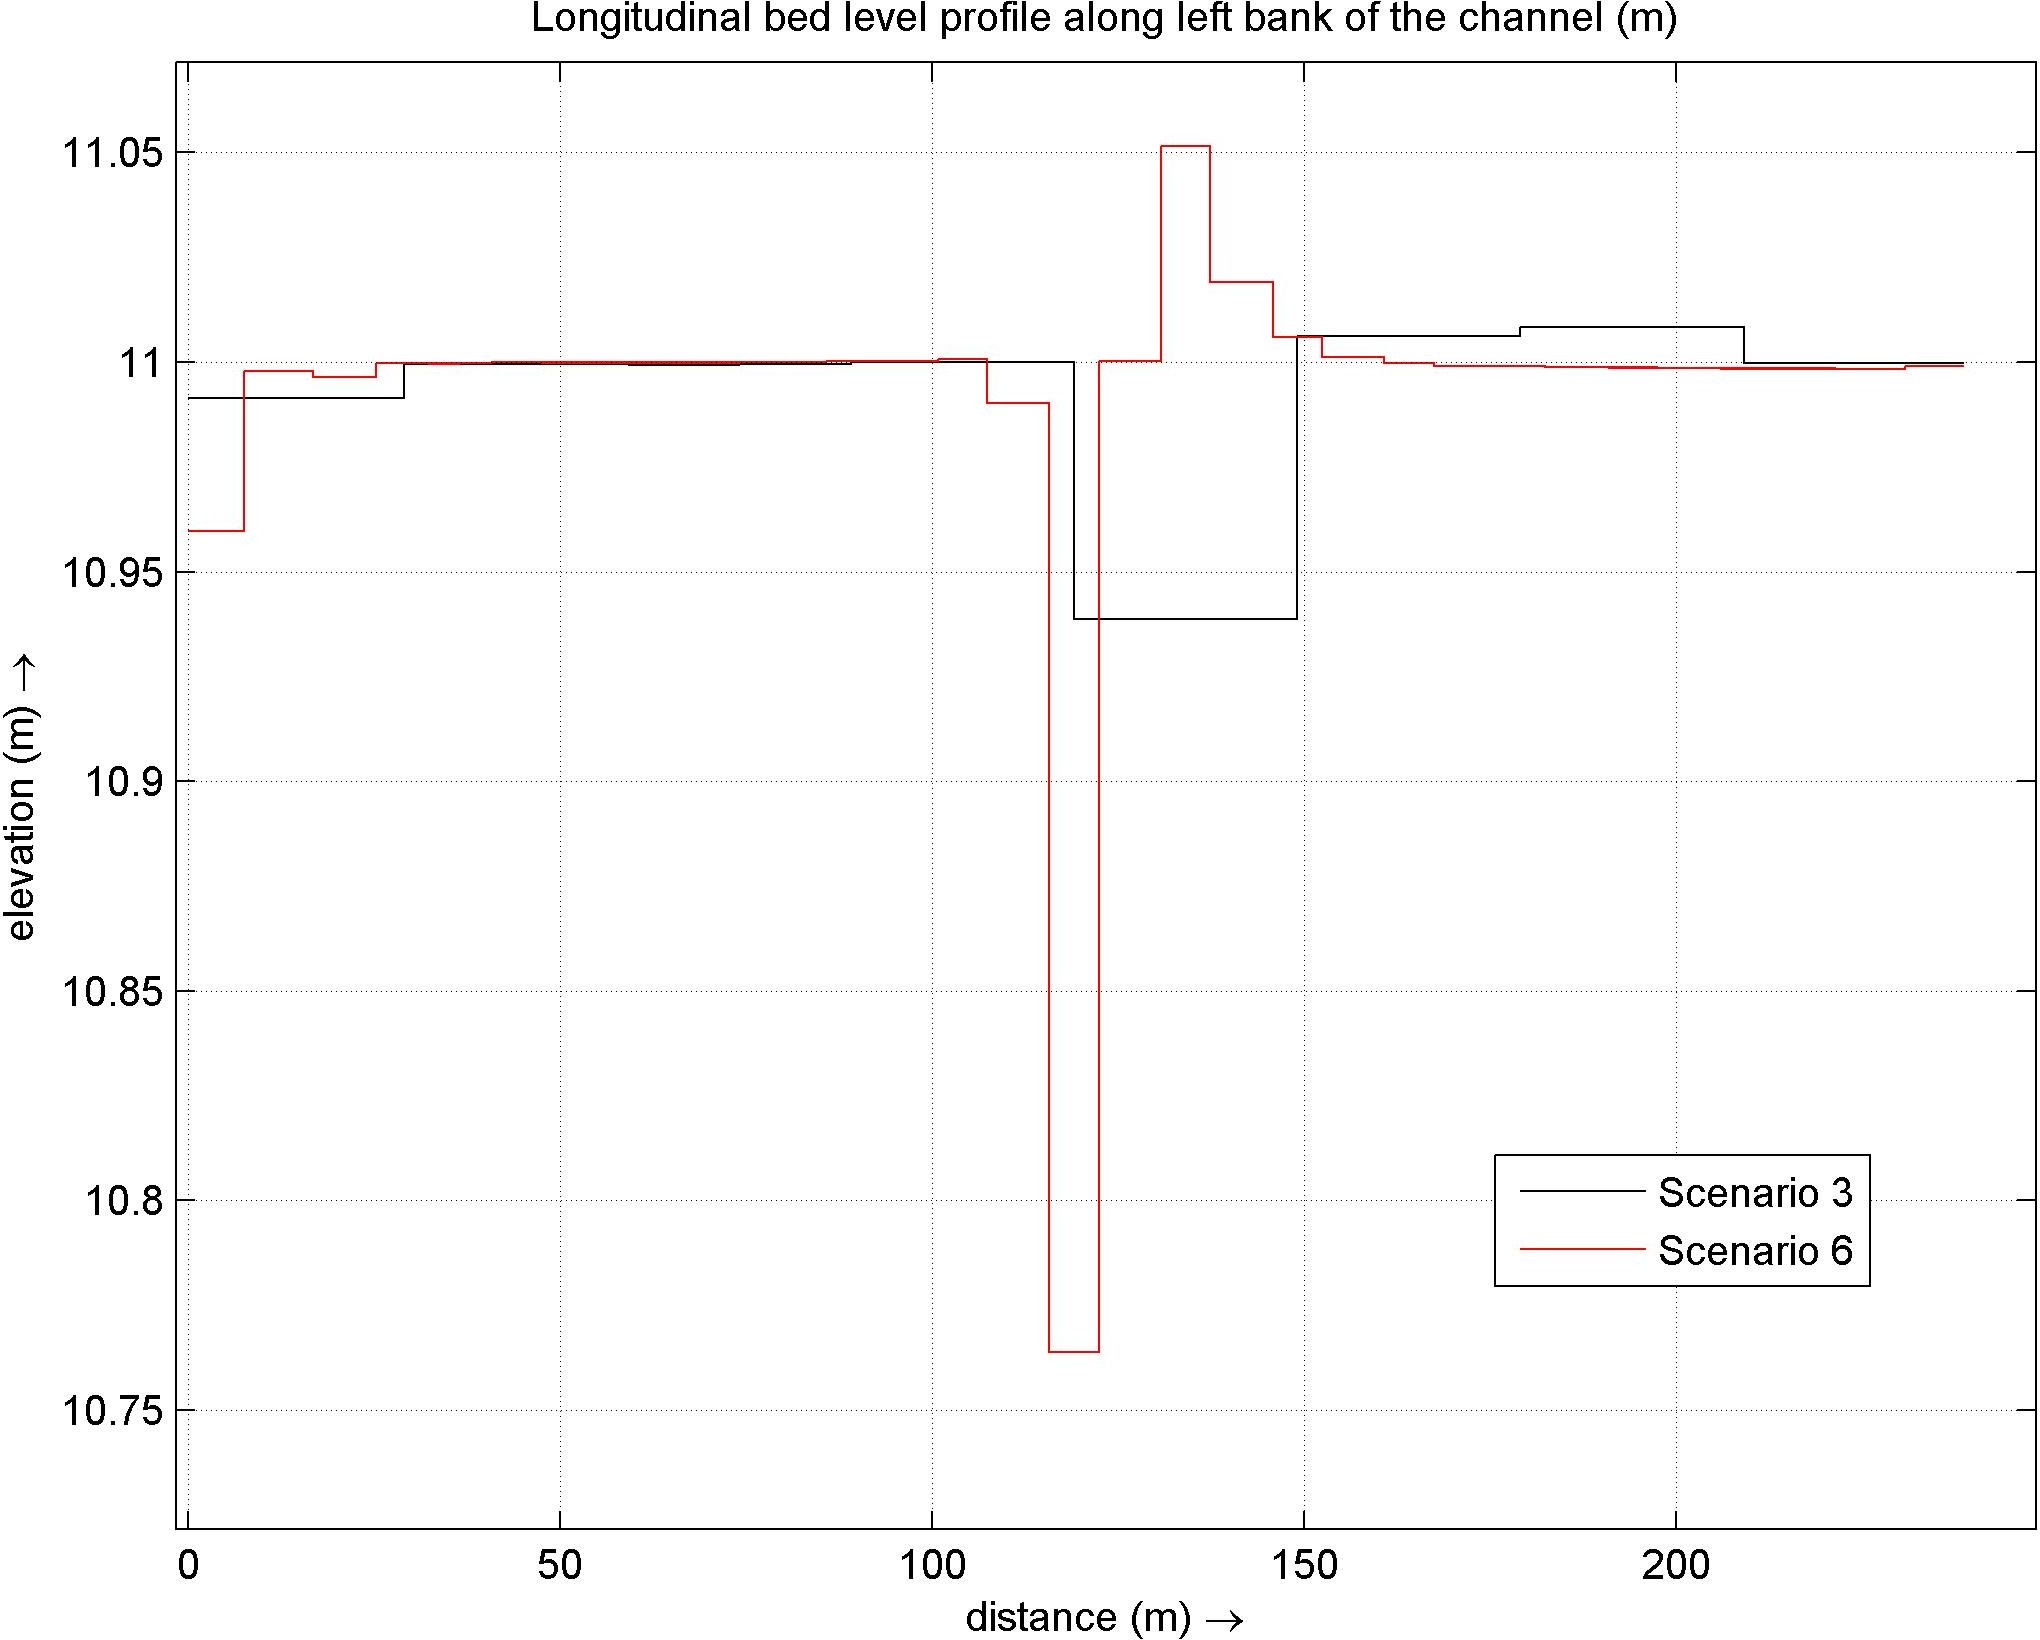
\includegraphics[width=0.8\columnwidth]{figures/BedlevelSc3-6-left.jpg} 
	\end{subfigure}
\end{center}
\caption{Longitudinal profiles of bed level changes along the channel center (upper plot) and the left parts (lower part) for the models with structured and unstructured grid}
\label{fig:1.10}
\end{figure}

\begin{figure}[h!]
	\begin{center}
		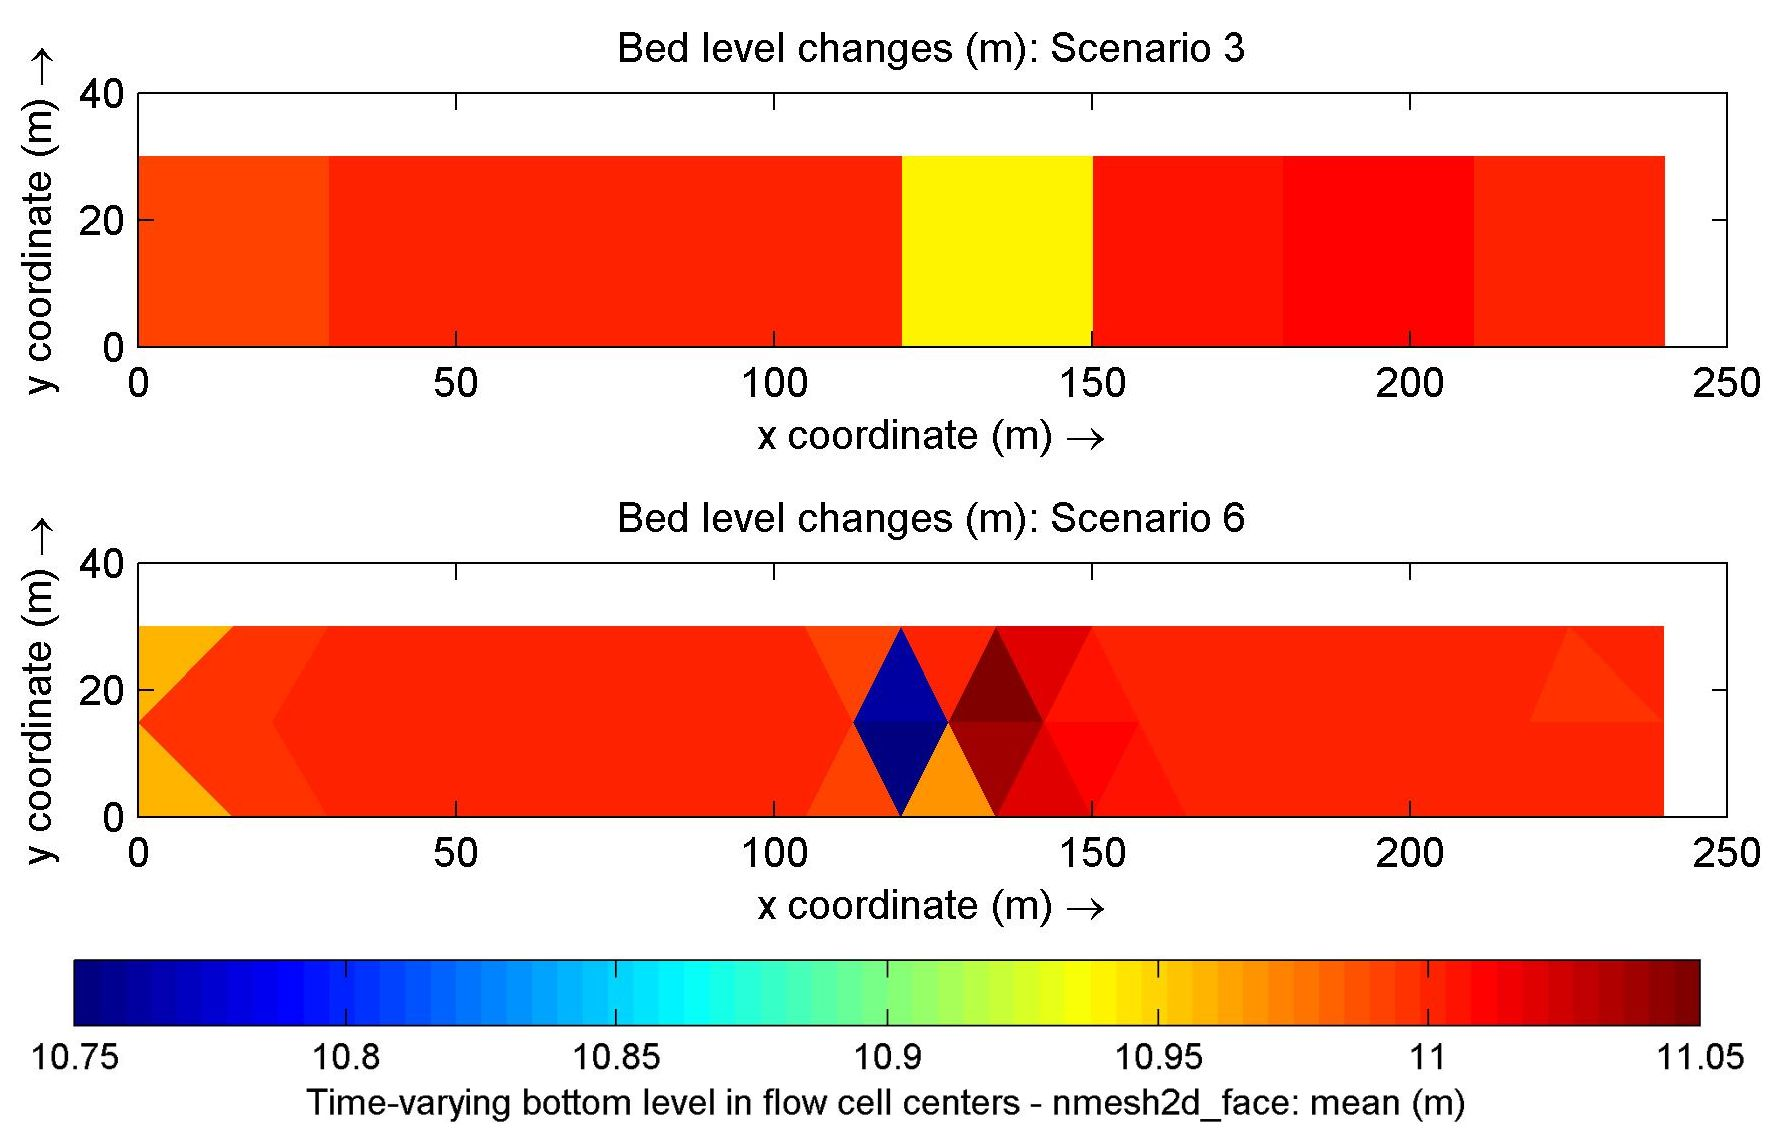
\includegraphics[width=0.8\columnwidth]{figures/BL-Combined.jpg} 
	\end{center}\caption{Bed level changes for structured (upper plot) and unstructured grid (lower plot). The location of the weir is similar to that, shown in Figure \ref{fig:1.9} \label{fig:1.11}}
\end{figure}

\begin{figure}[h!]
	\begin{center}
		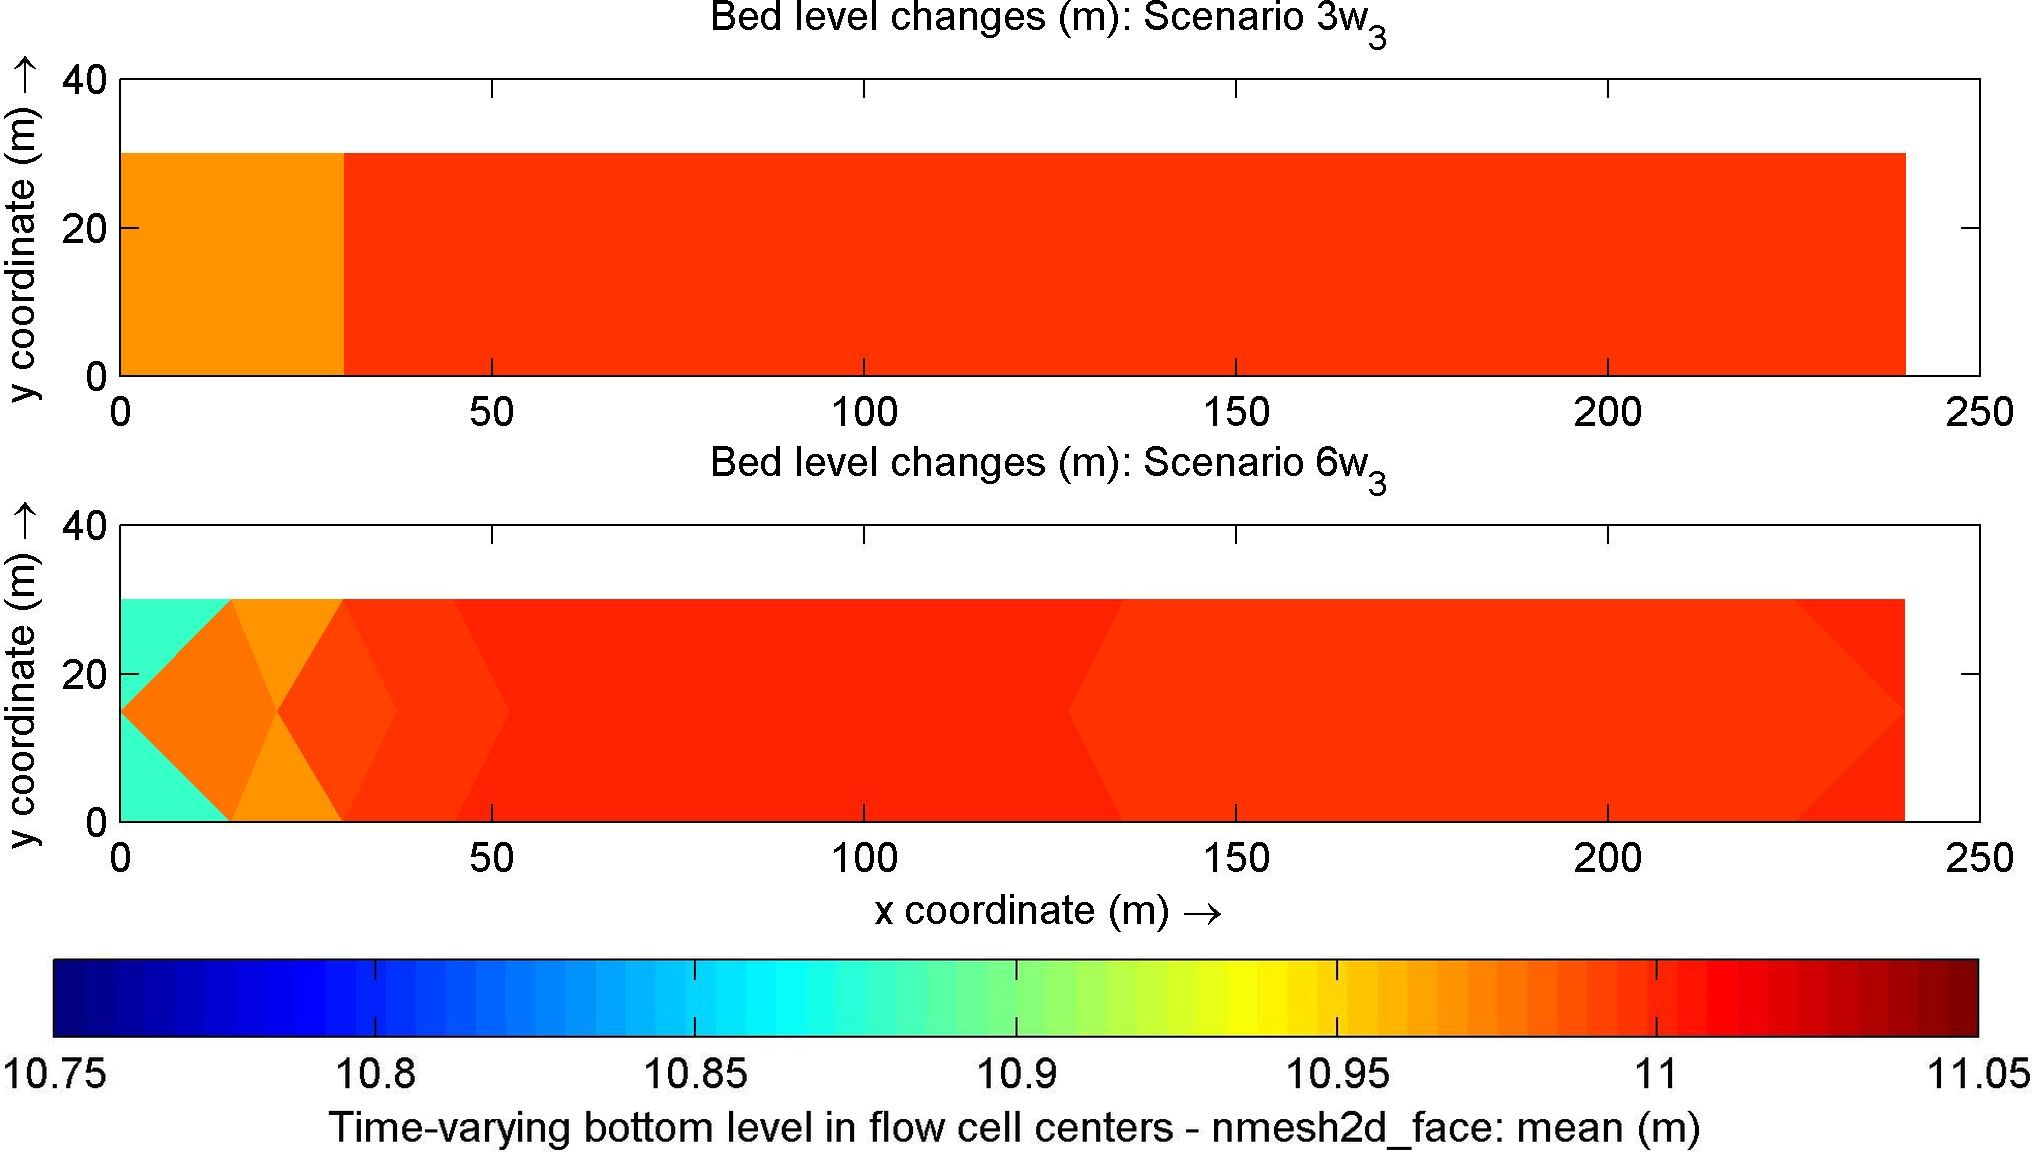
\includegraphics[width=0.8\columnwidth]{figures/BL-Combinedw3.jpg} 
	\end{center}\caption{Bed level changes for structured (upper plot) and unstructured grid (lower plot) for the scenarios under the condition of no weir treatment \label{fig:1.12}}
\end{figure}

\begin{figure}[h!]
	\begin{center}
		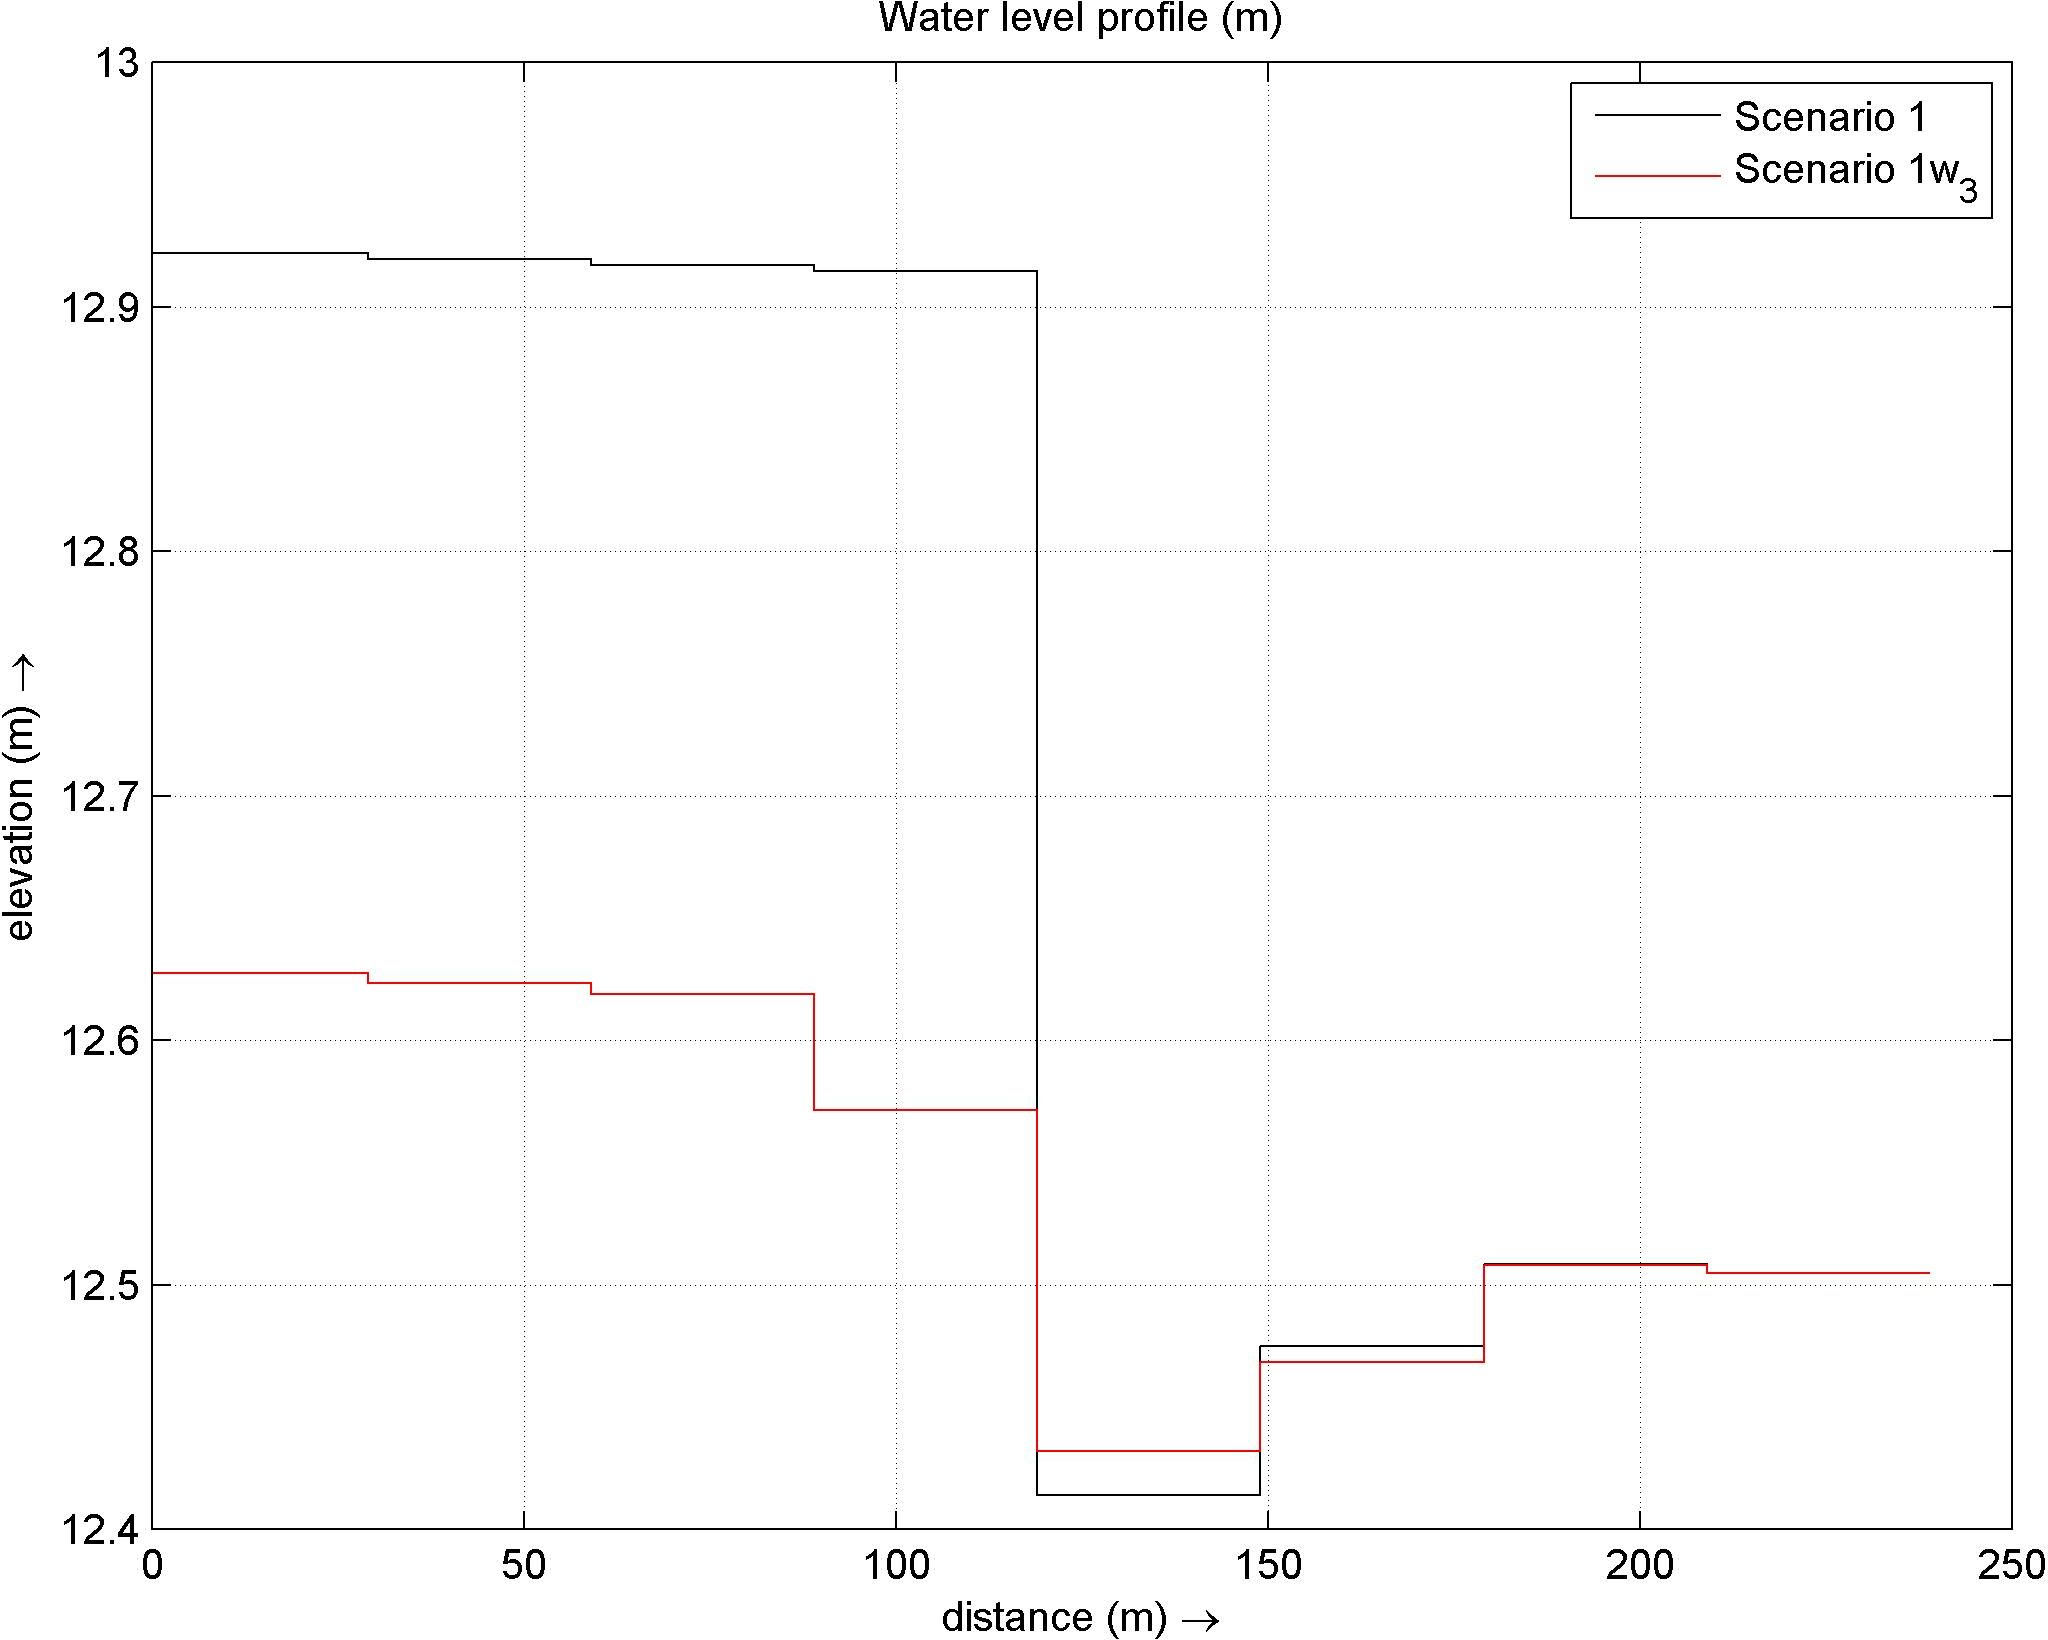
\includegraphics[width=0.8\columnwidth]{figures/WL-Sc1Sc1w1.jpg} 
	\end{center}\caption{Water level for scenarios with different weir input parameters for hydrodynamic simulation (model with structured grid) \label{fig:1.13}}
\end{figure}

\begin{figure}[h!]
	\begin{center}
		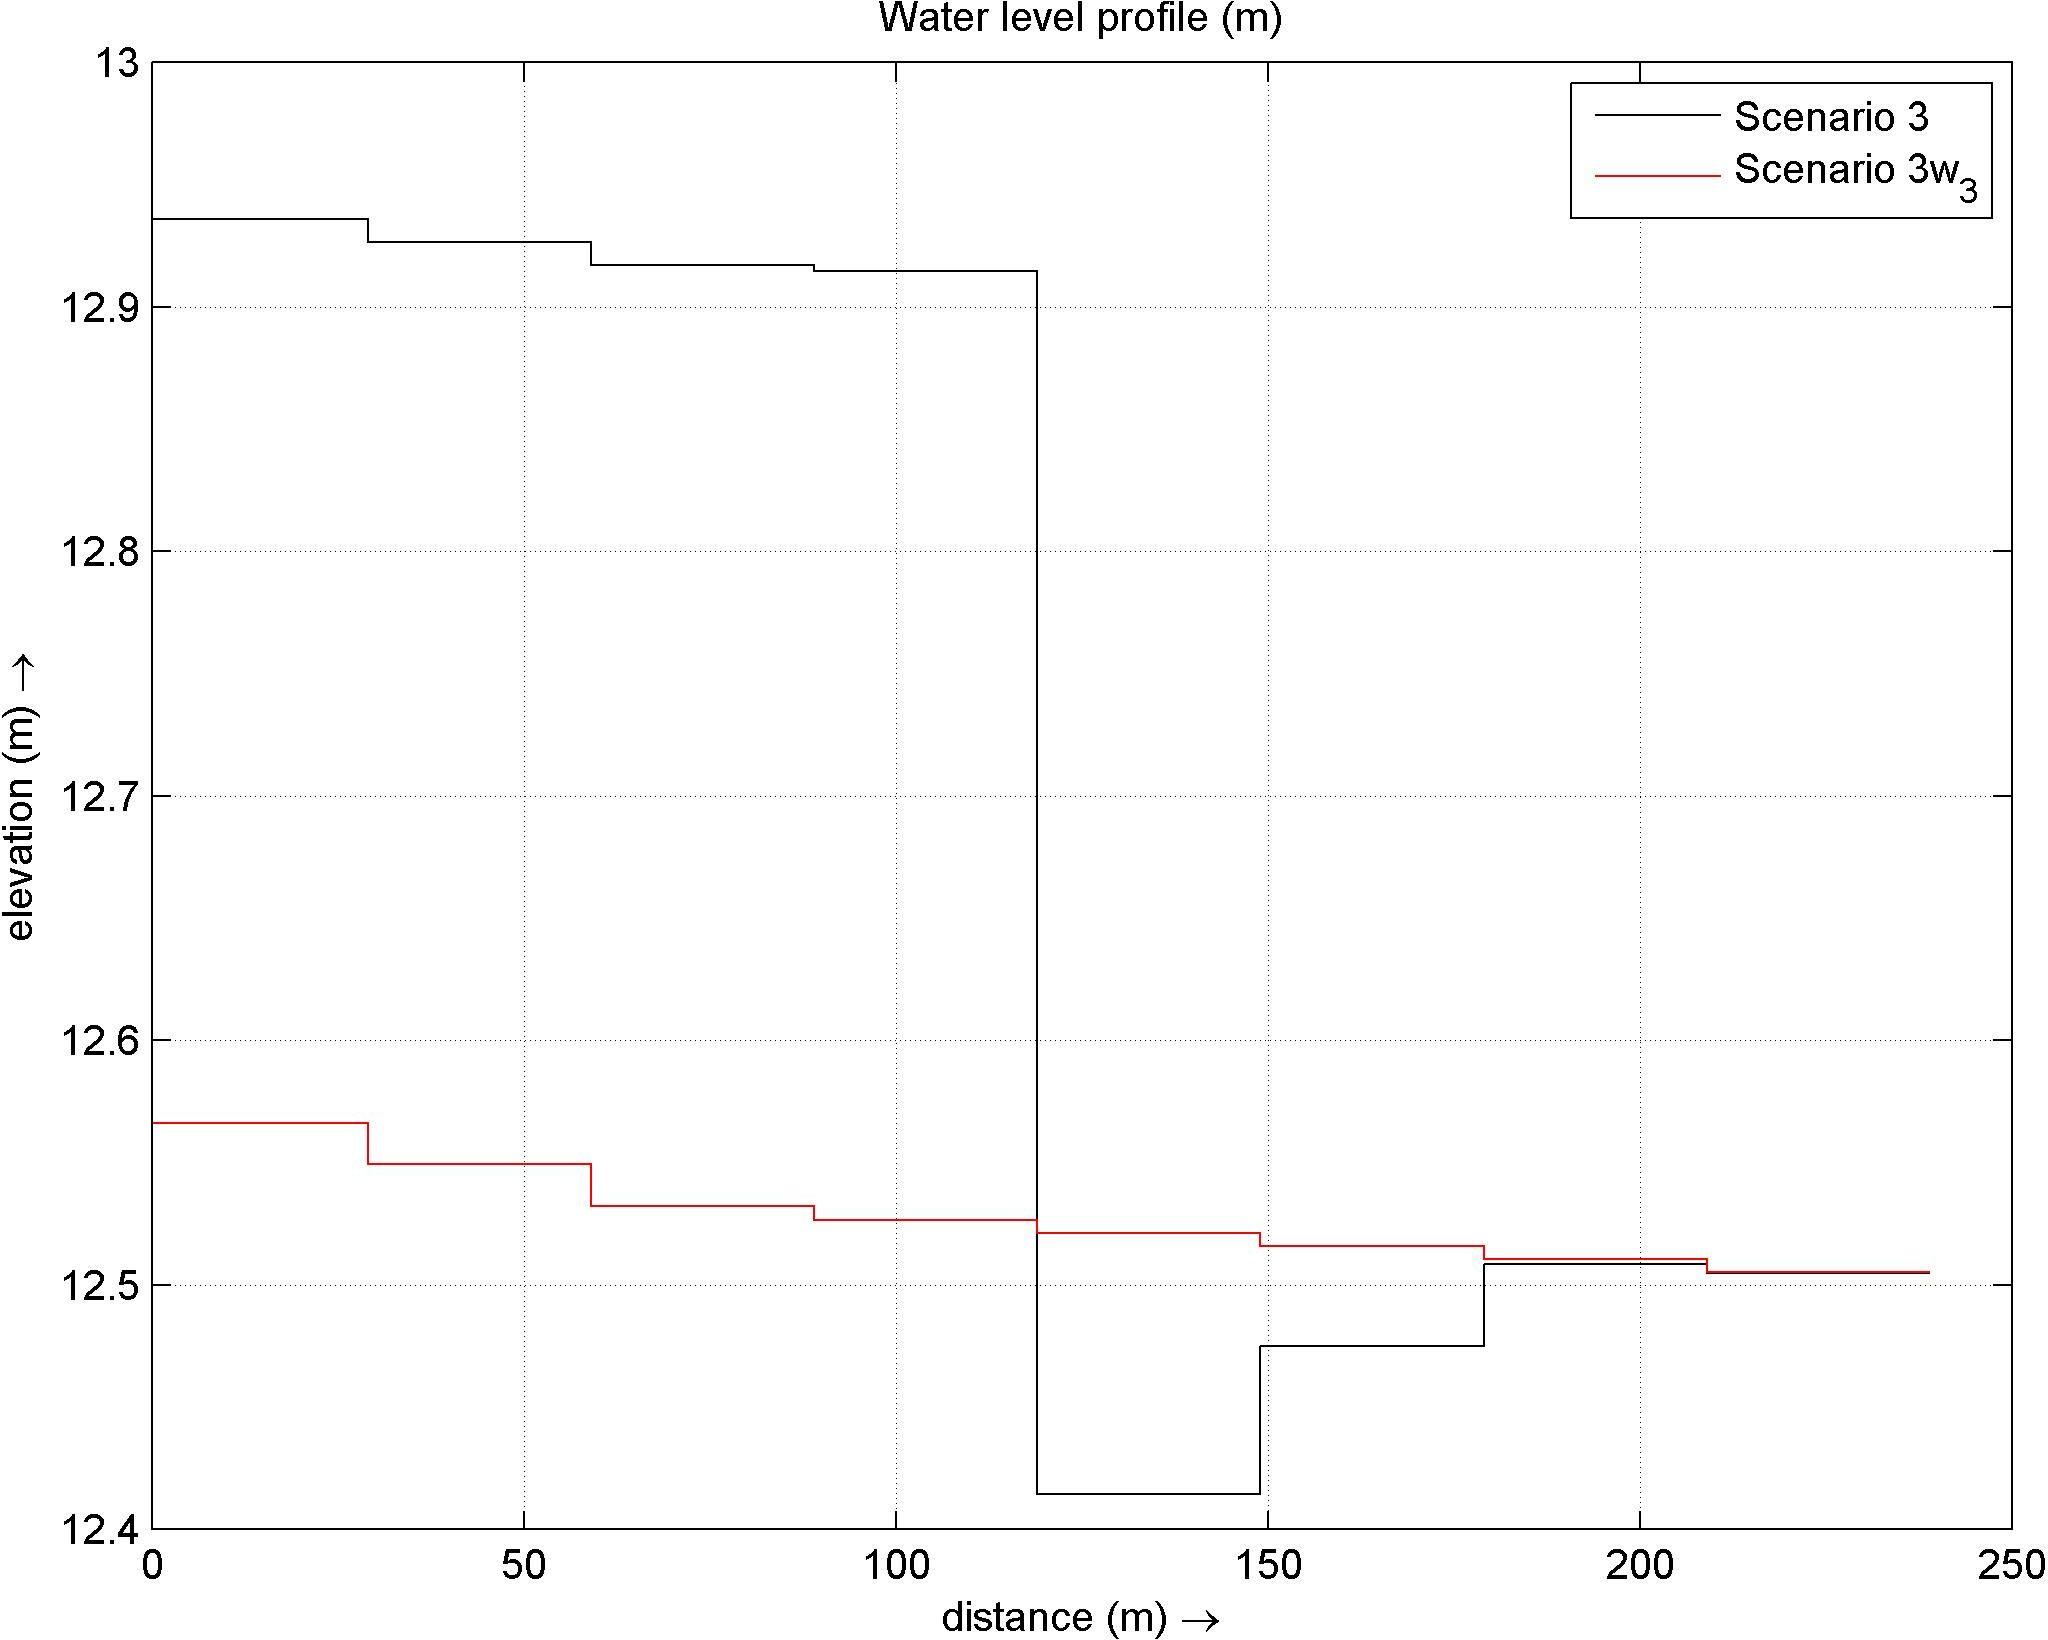
\includegraphics[width=0.8\columnwidth]{figures/WL-Sc3Sc3w3.jpg} 
	\end{center}\caption{Water level for scenarios with different weir input parameters for hydrodynamic simulation (model with structured grid) \label{fig:1.14}}
\end{figure}

\begin{figure}[h!]
	\begin{center}
		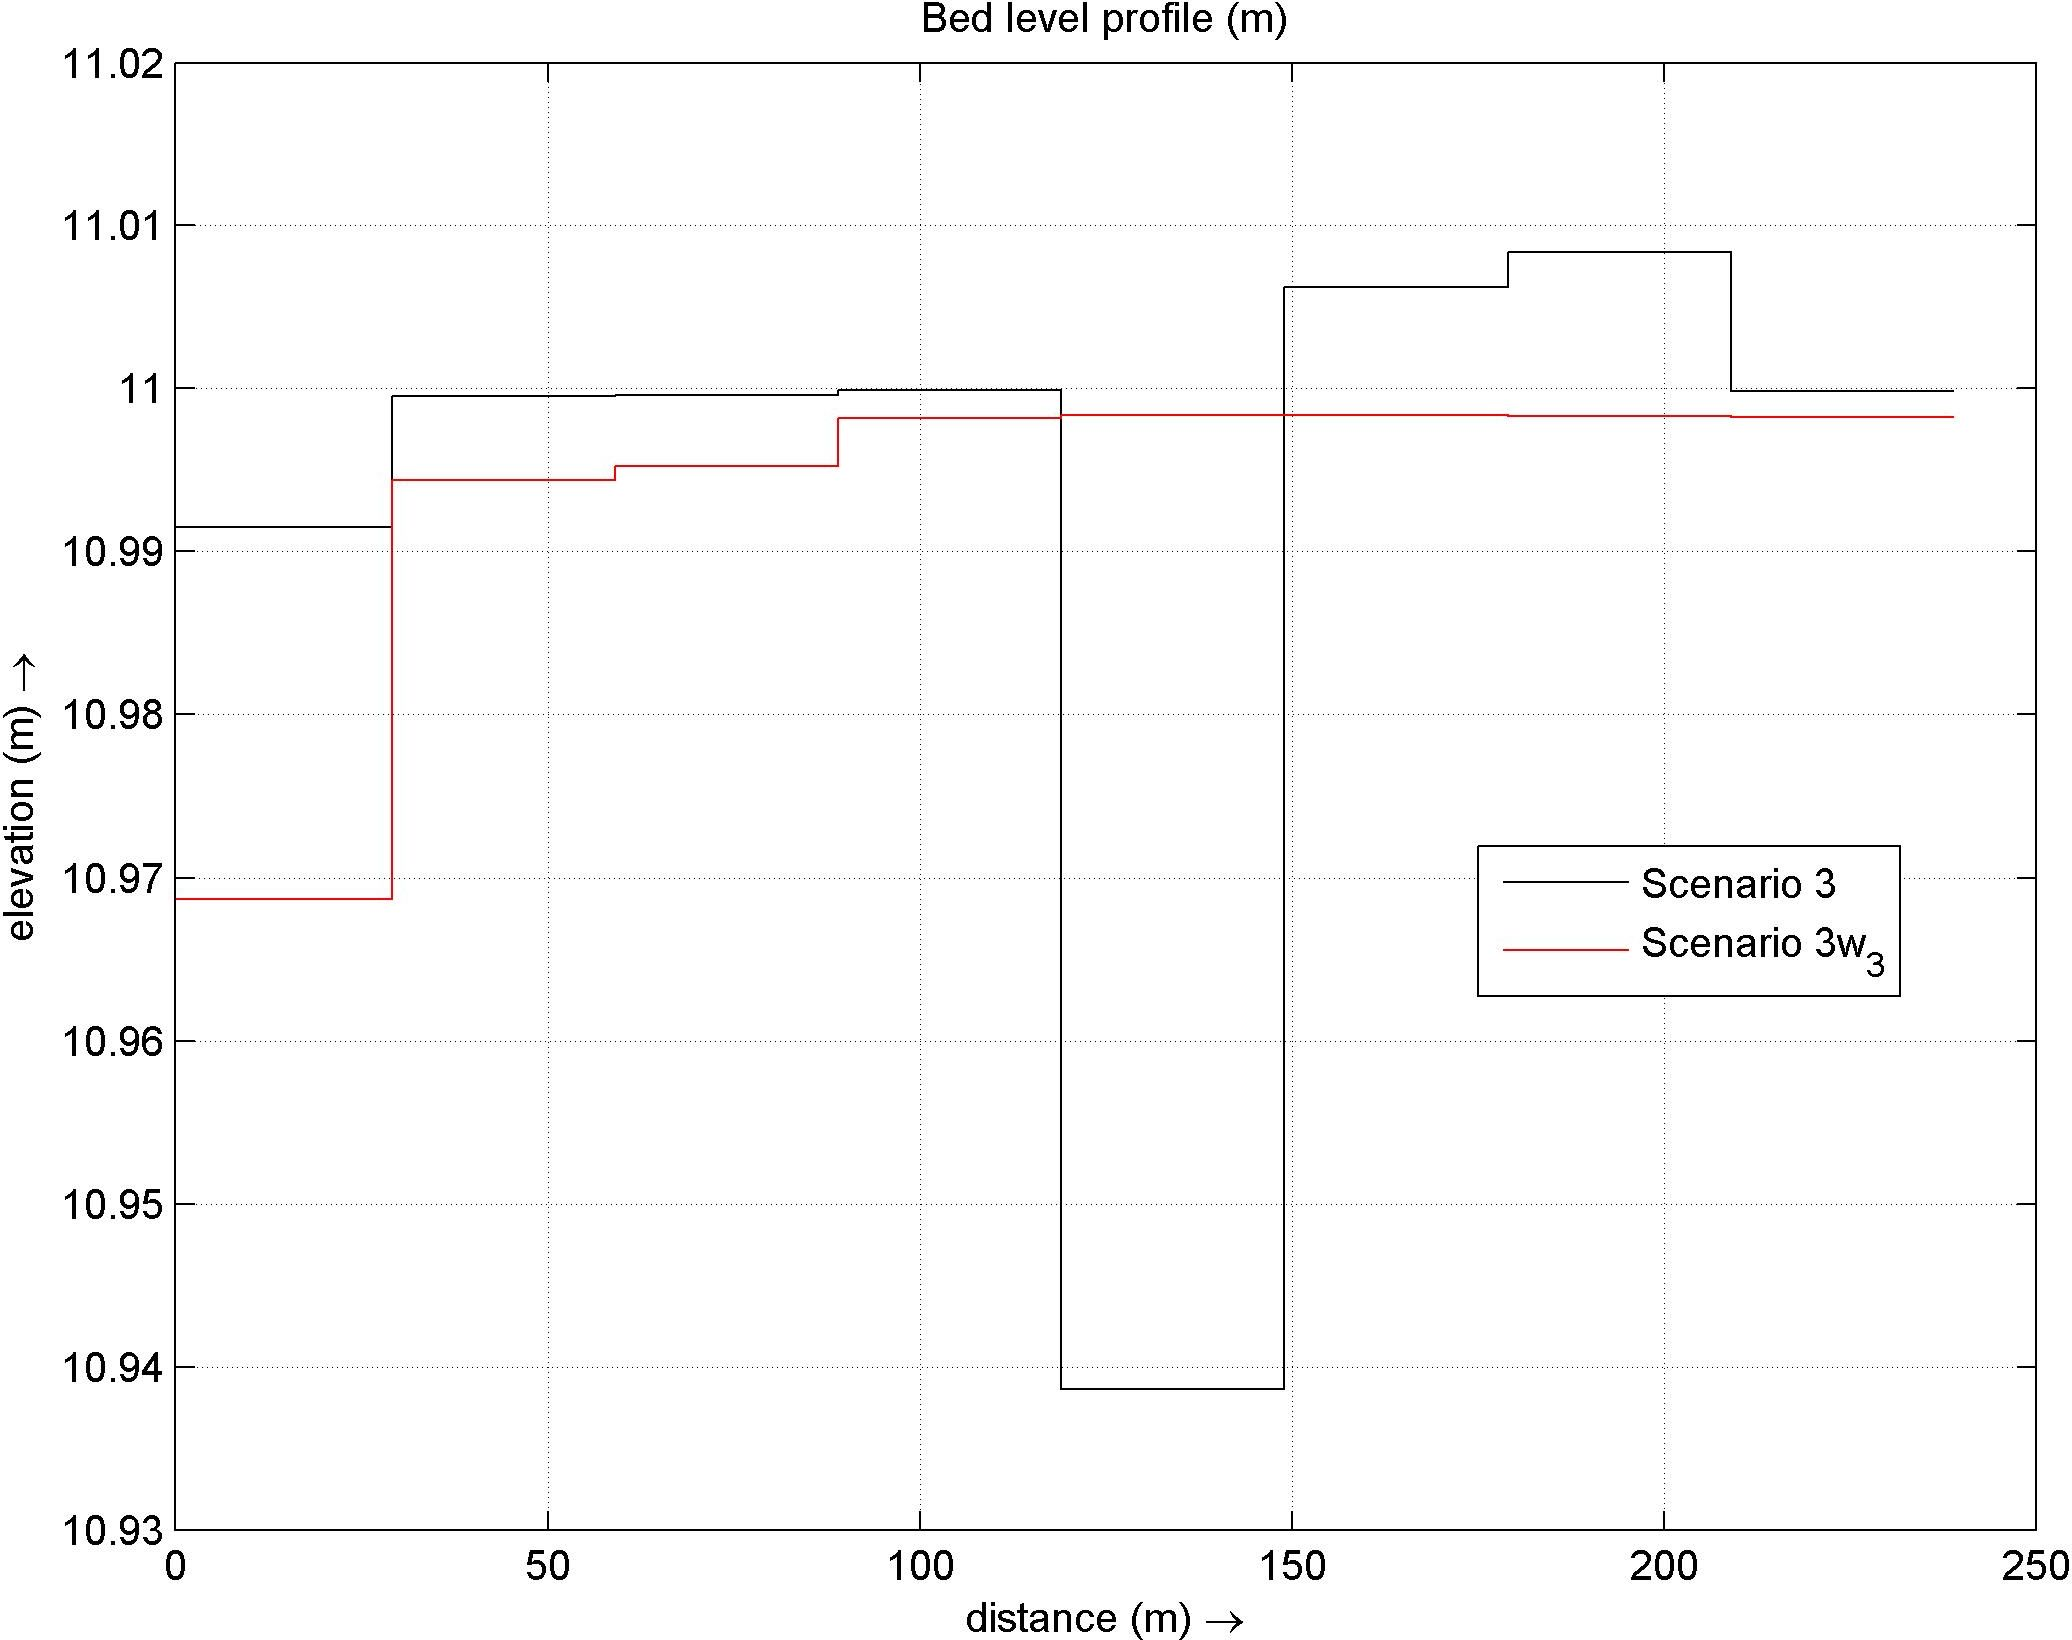
\includegraphics[width=0.8\columnwidth]{figures/BL-Sc3Sc3w3.jpg} 
	\end{center}\caption{Bed level changes for scenarios with different weir input parameters for morphologic simulation (model with structured grid) \label{fig:1.15}}
\end{figure}

\begin{figure}[h!]
	\begin{center}
		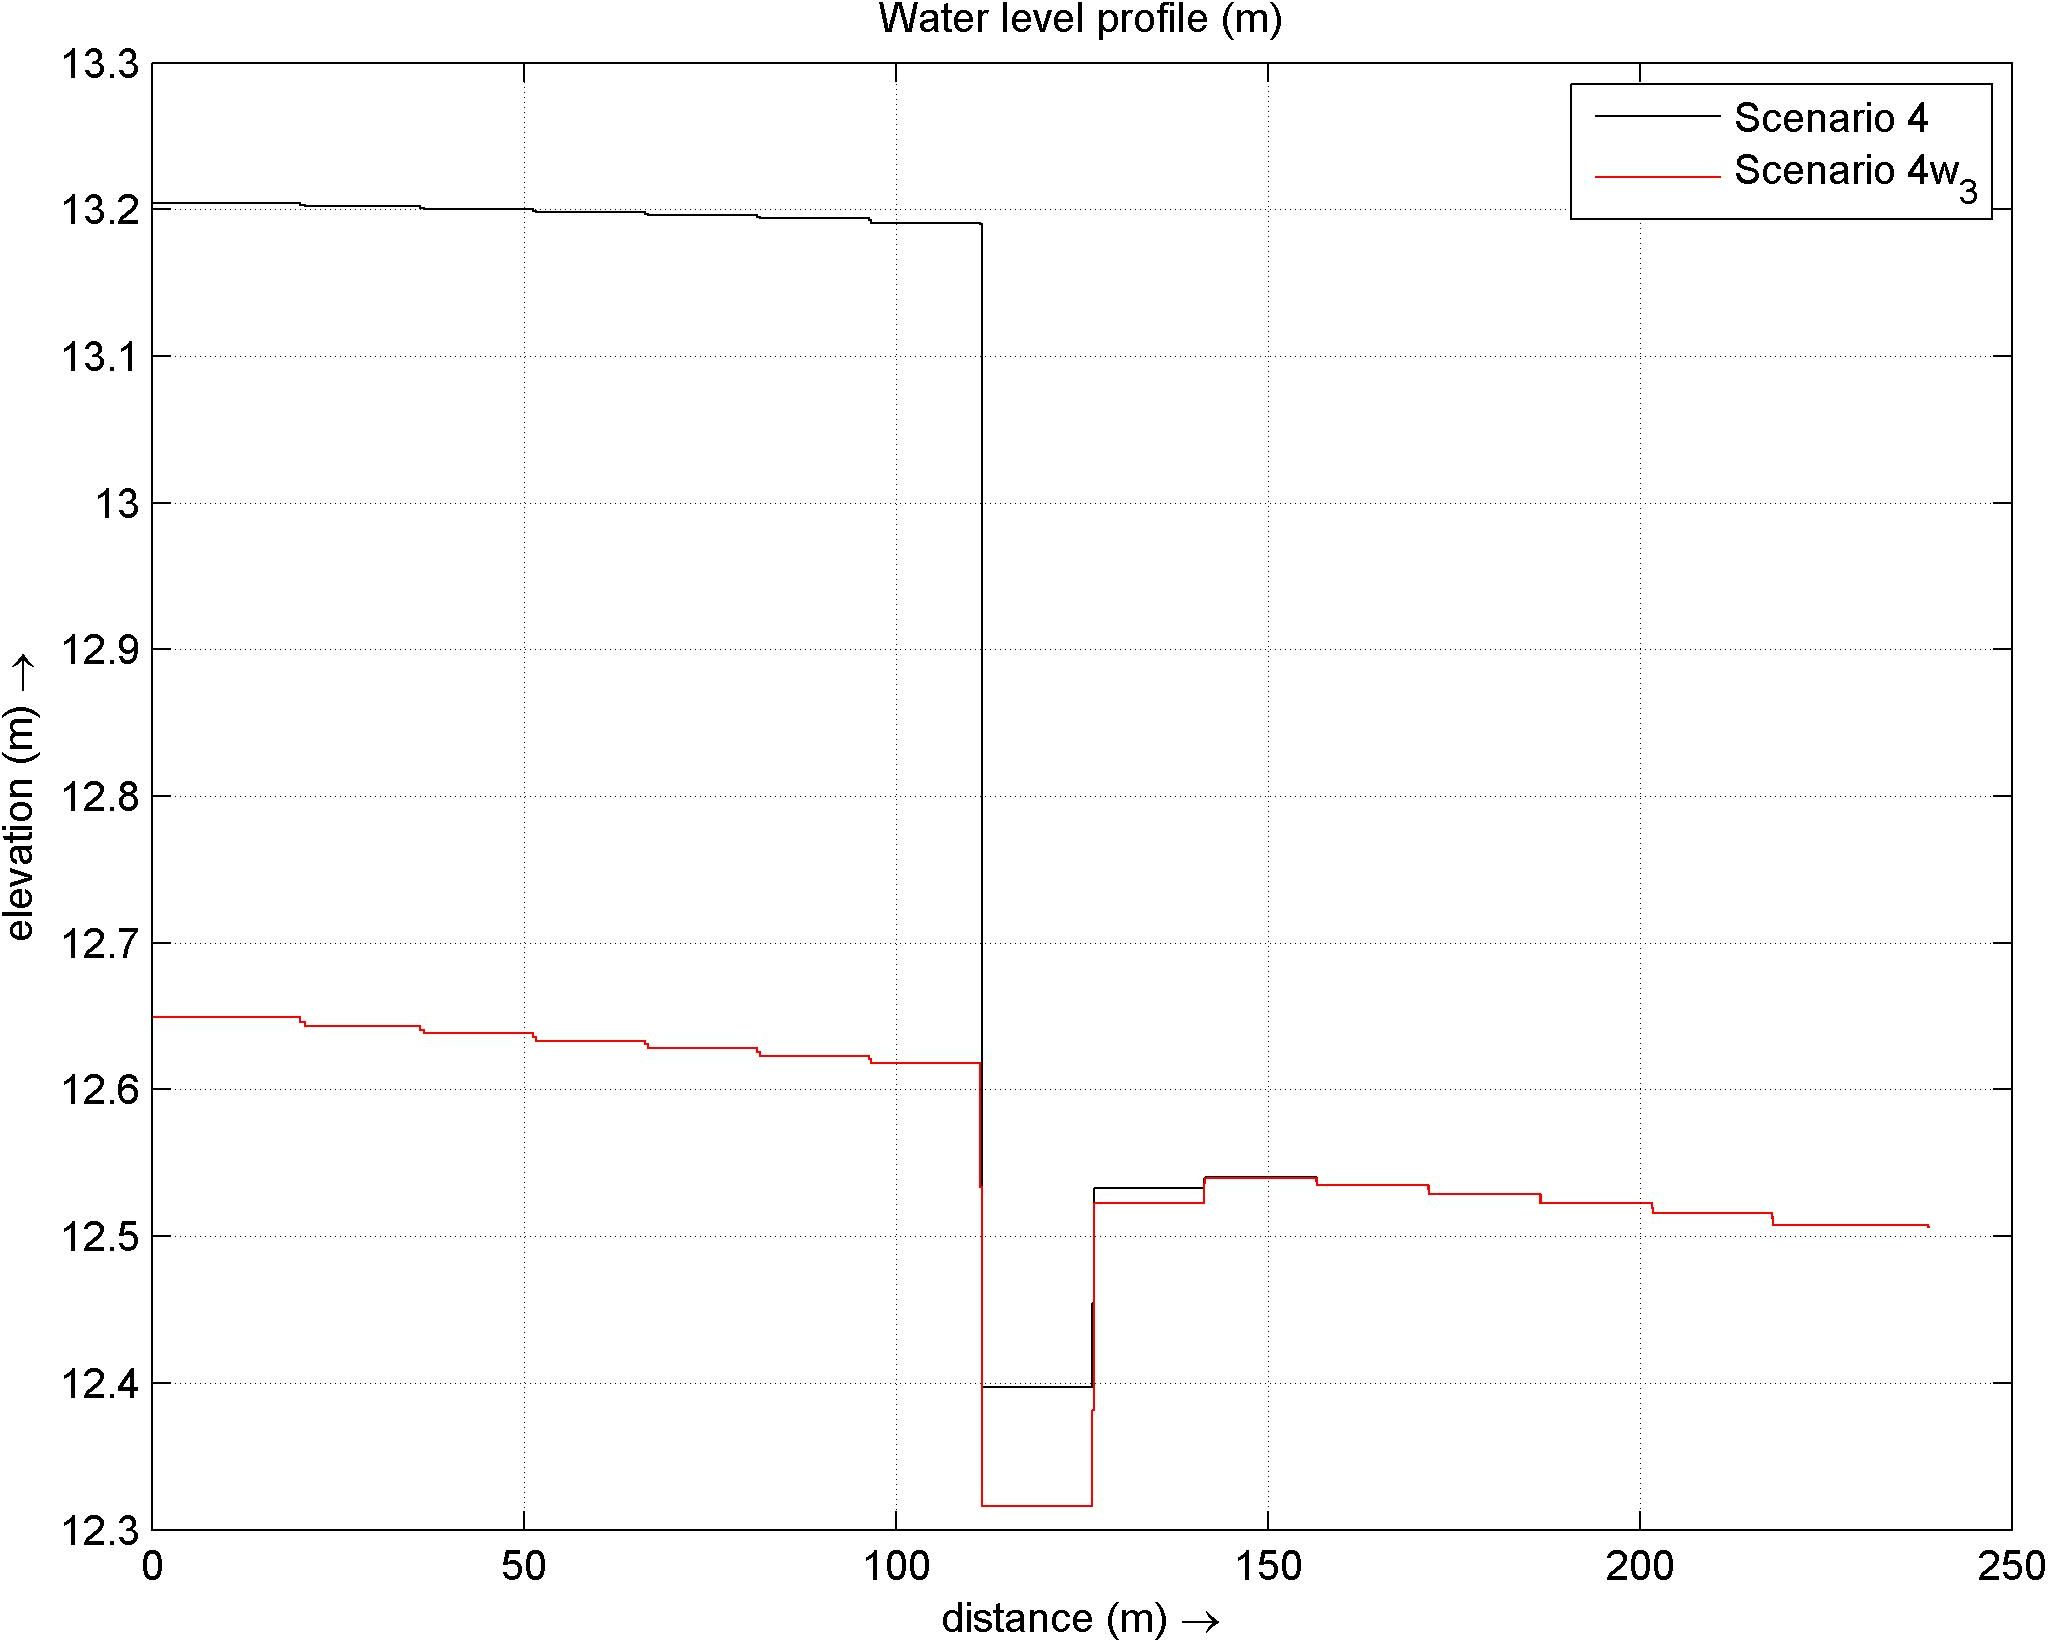
\includegraphics[width=0.8\columnwidth]{figures/WL-Sc4Sc4w3.jpg} 
	\end{center}\caption{Water level for scenarios with different weir input parameters for hydrodynamic simulation (model with unstructured grid) \label{fig:1.16}}
\end{figure}

\begin{figure}[h!]
	\begin{center}
		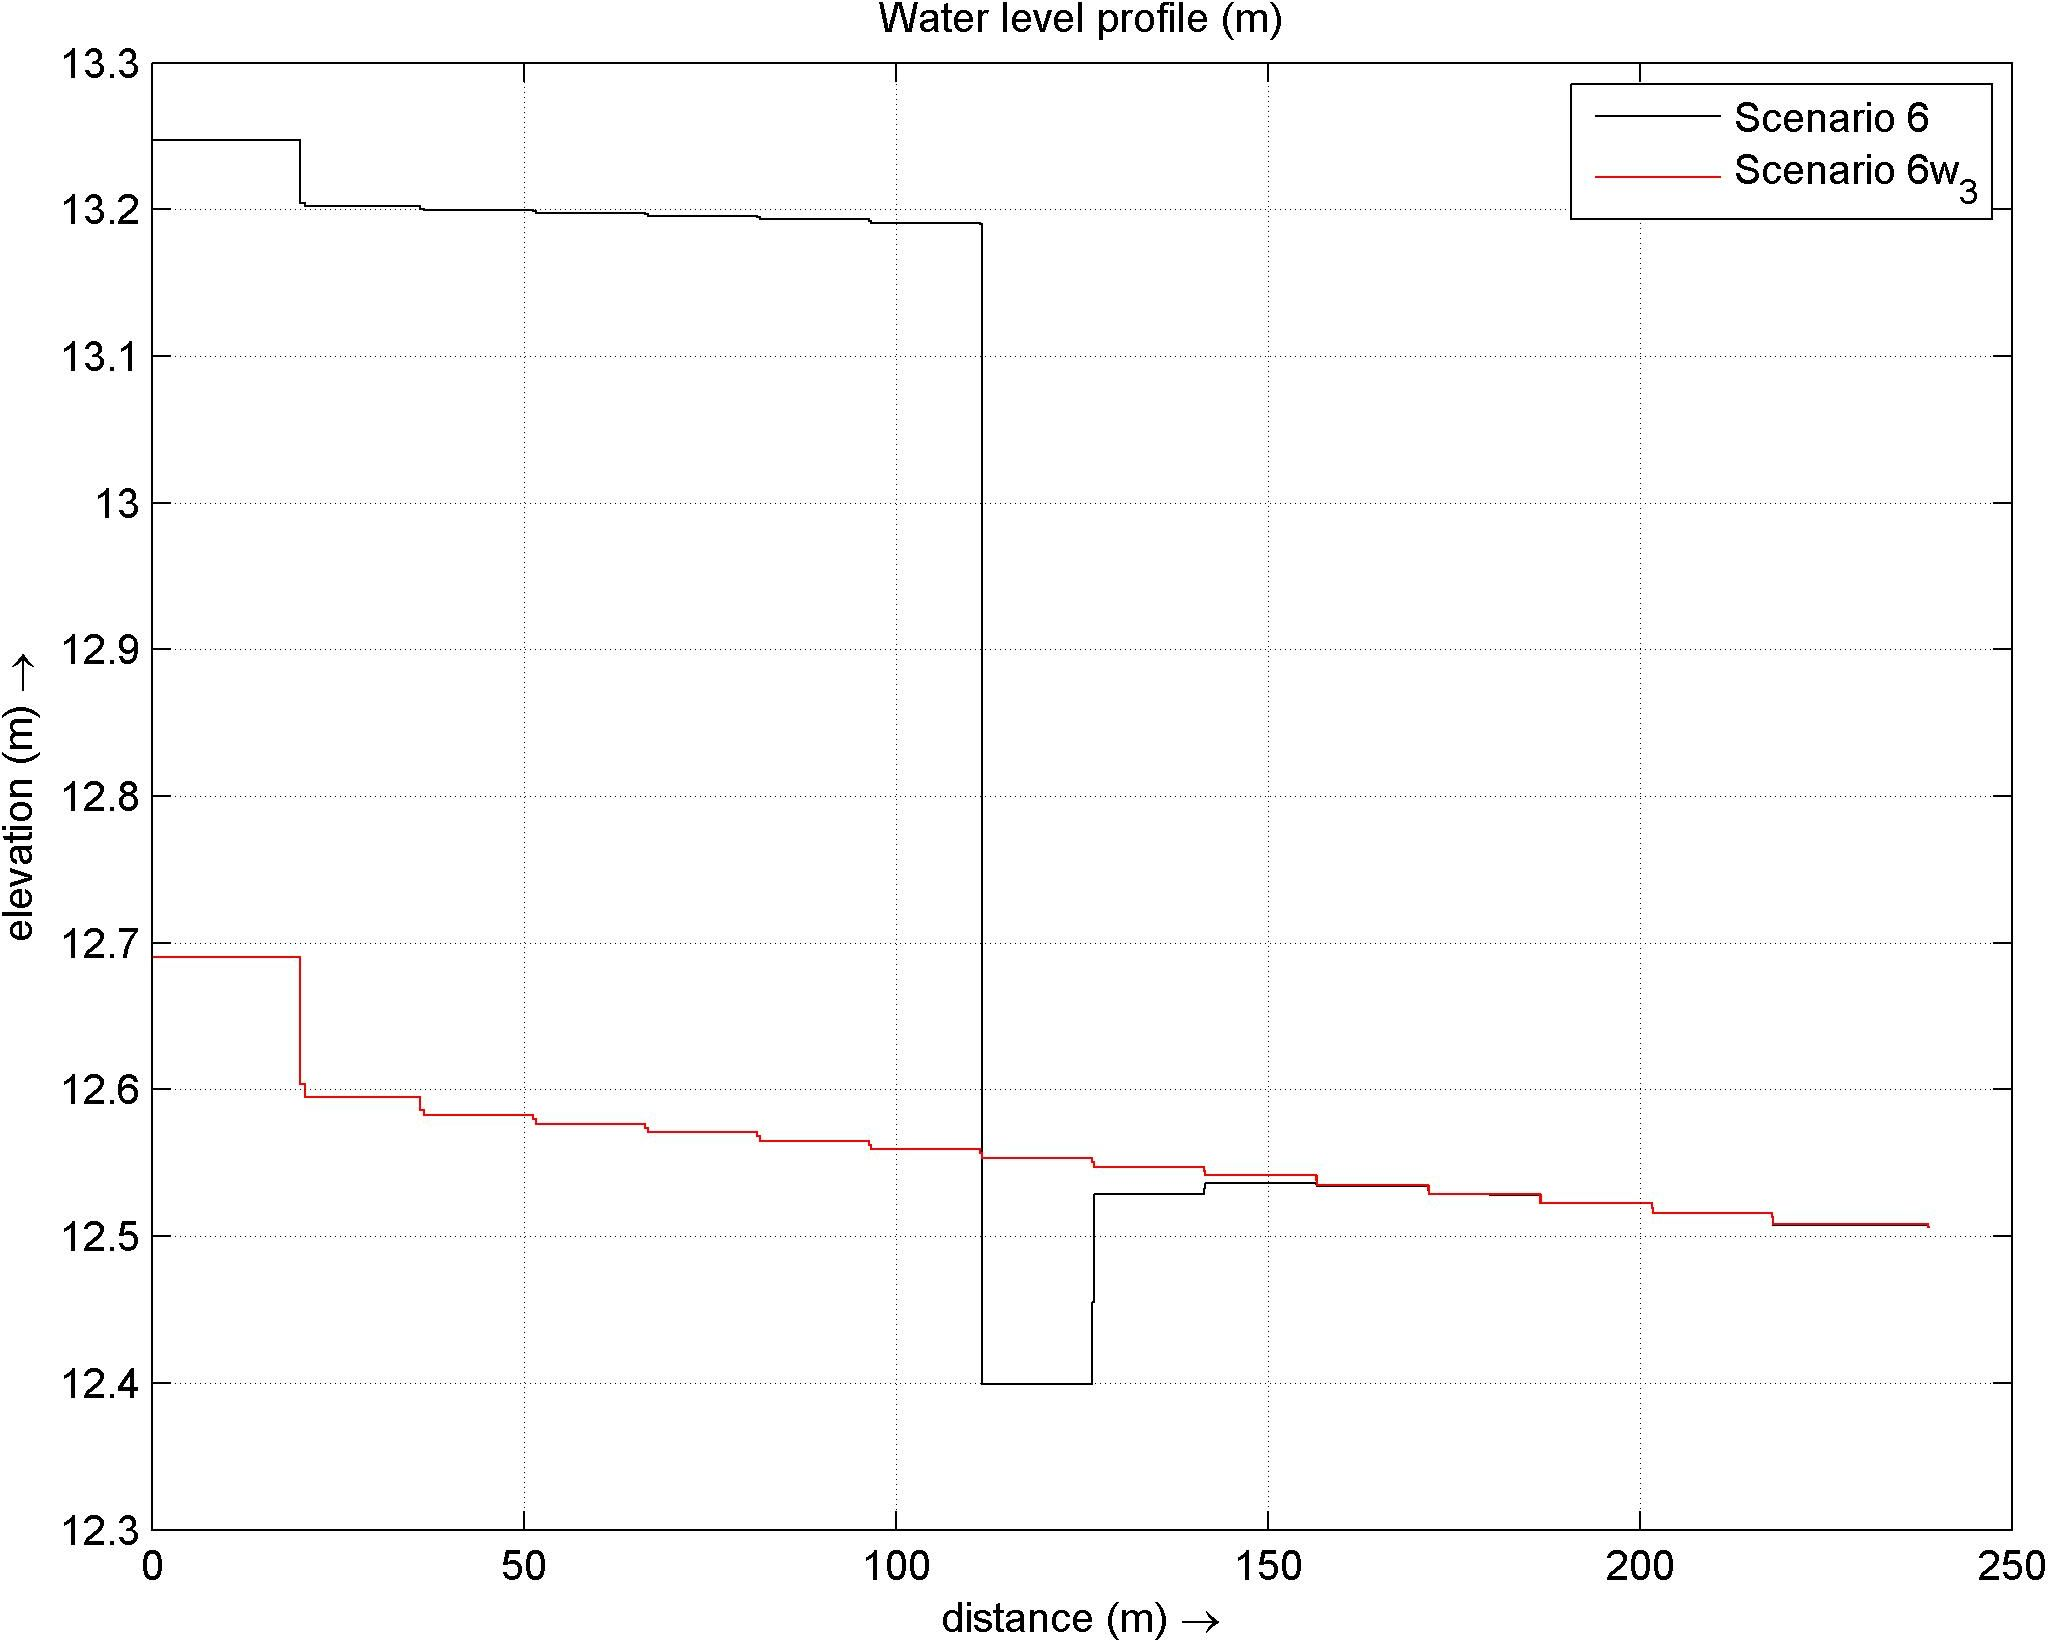
\includegraphics[width=0.8\columnwidth]{figures/WL-Sc6Sc6w3.jpg} 
	\end{center}\caption{Water level for scenarios with different weir input parameters for morphologic simulation (moel with unstructured grid) \label{fig:1.17}}
\end{figure}

\paragraph*{Results}
Following are the results of the test simulations and their comparison:

\begin{itemize}

\item	There is no difference between Scenario 1 and 2, 1w1 and 2w1 and 1w2 and 2w2. This implies that the condition for no bed level update in morphological file gives same result as hydrodynamics. The same is valid for the model with unstructured grid, i.e. for scenarios 4 and 5 as well as 4w1 and 5w1. 
\item	The differences between hydrodynamic and morphological test simulations with weir (generated using DeltaShell) are shown in Figure\ref{fig:1.2} - Figure \ref{fig:1.3} and Figure \ref{fig:1.4} - Figure \ref{fig:1.5}  for the models with structured and unstructured grid respectively. The results reflect the differences due to morphological changes realistically. However, the results are different for the models with structured and unstructured grid. This appears to be due to the fact that the weir is projected on to the grid differently, particularly deviated significantly in case of unstructured grid due to large grid resolution and orientation. In case of unstructured grid, the weir is not straight across the channel as in case of structured grid (shown in Figure \ref{fig:1.9} and mentioned below as well).  
\item	Comparison between model results with structured and unstructured grid (i.e., comparison between scenarios 1 and 4, 2 and 5 and 3 and 6) is depicted in Figure \ref{fig:1.6}, Figure \ref{fig:1.7} and Figure \ref{fig:1.8} respectively. The result shows that there are some differences in water level profiles. Figure 1.9 gives spatial impression of the water level differences, which can essentially be attributed to the effect of the grid on weir orientation (due to projection of the weir on to the unstructured grid as depicted in Figure \ref{fig:1.9}). 
\item	The erosion-deposition pattern and magnitude are different for the models with structured and unstructured grid as shown in Figure \ref{fig:1.10} and Figure \ref{fig:1.11}. This can also be attributed to the difference in grid type and weir projection and orientation. It is to be noted that there is some erosion at the upstream boundary in case of unstructured grid. We have checked this also for the morphological simulation scenarios under the condition of no weir treatment (i.e. scenarios 3w3 and 6w3 for structured and unstructured models respectively). The result reveals that there is more erosion near the inflow boundary in case of unstructured grid (as shown in Figure \ref{fig:1.12}). So, this shall be explored further.   
\item	Scenarios with different input files for weir with and without additional parameters (i.e. sill depth at two sides) reveal some inconsistent result, particularly for hydrodynamic simulation (Scenario 1w3). The condition $“Sillheightmin” = 0.5$ in $*.mdu$ file and both sill depth = 0 in weir file should lead to no weir treatment. However, there is some energy loss as depicted in Figure \ref{fig:1.13} (although the weir effect is less comparing to Scenario 1). However, for morphological simulation with same condition (Scenario 3w3), the result looks consistent (i.e., no weir treatment, so no head loss as depicted in Figure \ref{fig:1.14}). The effect of weir input is reflected on the bed level changes as well, as shown in Figure \ref{fig:1.15}. This issue is same for the model with unstructured grid as well (depicted in Figure \ref{fig:1.16} and Figure \ref{fig:1.17}). The reason for these discrepancies is not clear and shall be explored further.  

\end{itemize}


\paragraph*{Conclusions}
This validation case shows that D-Flow FM is able to model morphology in combination with weirs. The morphology with \emph{BedUpd= false} does not influence the solution of the hydrodynamics.
However, following are some remarks and recommendations: 
\begin{itemize}
\item	In general, morphological models with weir have been found to be functioning as expected given the fact that the effect of weir on morphological changes appears to have been replicated qualitatively well. Although there is no assurance about their correctness in quantitative terms. 
\item	The main point to be mentioned is about the comparison between the models with structured and unstructured grid. Since the grid is too coarse, the weir is projected on to the unstructured grid differently than on structured grid. Therefore, it is not reliable to compare the results between these two models given the fact that both hydrodynamic and morphologic changes are predominantly affected by the weir orientation. 
\item	There is some inconsistency in model results associated with weir-related condition and parameters, namely $“Sillheightmin”$ in $“*.mdu”$ file and sill depth parameters in weir file. The weir treatment must be active only when $“Sillheightmin”$ is higher than the sill depth, specified in weir file (generated by DeltaShell). This is not always working and thus needs to be explored further. 
\item	There is some problem related to erosion near the inflow boundary, particularly for the unstructured model. This shall be explored further.  
\item	It should be noted that the resolution and orientation of unstructured grid is important to be considered, particularly for situations when there are structures with different orientation. This is even more vital for morphological computations. For real-world application with structures (like for Rhine branches), care must be taken while generating grid, since the orientation of the projected structures on to the grid must resemble reality as correctly as possible. This implies that structured grid must be used as much as possible, particularly for the main channel with dominant flow and morphological activities. 
\end{itemize}

\paragraph*{Version}
This test has been carried out with version D-Flow FM Version 1.1.188.47075.